%\renewcommand*\thechapter{\Alph{chapter}}

	\part*{Teil 1: Maß- und Integrationstheorie}


\chapter{Maßtheorie (Modellierung von Ereignissen und Wahrscheinlichkeiten)}
	\marginpar{\textcolor{red}{Vorlesung 1}}
Ma\ss - und Integrationstheorie bildet die formale Grundlage um zuf\"allige Experimente zu modellieren. In diesem ersten Teil der Vorlesungen beweisen wir alle notwendigen Theoreme. Nicht alles wird sp\"ater uneingeschr\"ankt wichtig sein, das Arbeiten mit den neuen Begriffen wird sich in zuk\"unftigen Vorlesungen aber auszahlen!


\section{$\sigma\text{-Algebren}$ und Maße - die Grundbegriffe der Stochastik}\label{sigmaalgebra}
Im Prinzip sind die kommenden f\"unf Vorlesungen total elementar, wir brauchen nur Kenntnisse \"uber Mengen, Folgen und Reihen. Die Vorlesung nutzt also nur Kenntnisse der Analysis 1. Dennoch wird euch der Inhalt zun\"achst schwer fallen weil wir Mengensysteme nicht visualisieren k\"onnen und daher viel abstrakt denken m\"ussen. Es wird sehr wichtig sein, die richtigen Beispiele im Kopf zu haben. Diese sollten nicht zu einfach sein, weil sonst der Gro\ss teil der Schwierigkeiten nicht erkannt werden kann. F\"ur $\sigma$-Algebren sollten wir m\"oglichst schnell die Borel-$\sigma$-Algebra als Standdardbeispiel im Kopf halten, f\"ur Ma\ss e das Lebesgue-Ma\ss. Endliche Beispiele werden wir nur ganz kurz als Motivation der Ma\ss theorie f\"ur Stochastik betrachten (W\"urfeln, M\"unzwurf, etc.), solche Beispiele bringen leider nicht viel um die Konzepte der Wahrscheinlichkeitstheorie richtig zu verstehen.\smallskip

Im Folgenden sei $\Omega \neq \emptyset $ immer eine beliebige Grundmenge. Für $A \subseteq \Omega$ bezeichnet $A^C$ immer das Komplement von A in $\Omega$, d. h. $A^C = \{ w \in \Omega \: | \: w \notin A \}$. $\mathcal{P}(\Omega)$ bezeichnet die Potenzmenge von $\Omega$ (inklusive $\emptyset$ und $\Omega$), eine Teilmenge von $\mathcal{P}(\Omega)$ ist also eine Menge von Mengen (man sagt auch Mengensystem).



\begin{deff} \link{https://www.youtube.com/watch?v=x7rMsOaujL8&list=PLy5qRKPWp6SBwfc1kn-b66cWc84cOgvqZ&index=3&t=458s}
	$\mathcal{A} \subseteq \mathcal{P}(\Omega)$ heißt $\sigma\text{-Algebra}$, falls
	\begin{enumerate}[label=(\roman*)]
		\item $\Omega \in \mathcal{A}$,
		\item $A \in \mathcal{A} \Rightarrow A^C \in \mathcal{A}$, das nennt man auch abgeschlossen (oder stabil) unter Komplementbildung,
		\item $A_{1},A_{2},... \in \mathcal{A} \Rightarrow \bigcup\limits_{k=1}^{\infty}A_k \in \mathcal{A}$, das nennt man auch abgeschlossen (oder stabil) unter abzählbarer Vereinigung.
	\end{enumerate}
	Elemente von $\mathcal{A}$ heißen \textbf{messbare Mengen}. Ist $\mathcal{A} \subseteq \mathcal{B}$ und $\mathcal{A}, \mathcal{B}$ sind $\sigma\text{-Algebren}$, so nennt man $\mathcal{A}$ $\text{Unter-}\sigma\text{-Algebra}$ von $\mathcal{B}$.
\end{deff}
Die Stabilit\"at f\"ur Vereinigungen gilt auch, wenn man nur endlich viele messbare Mengen vereinigen will. Dazu nutzt man einfach folgenden Trick: Wenn man messbare Mengen $A_1,...,A_N$ vereinigen m\"ochte, so setzt man $A_{N+1}=A_{N+2}=... =\emptyset$ und beachtet, dass damit wegen der $\sigma$-Additivit\"at $\cup_{k=1}^N A_k=\cup_{k=1}^\infty A_k\in \mathcal A$ gilt. Merkt euch solche kleinen Tricks, der selbe Trick taucht gleich nochmal auf.
\begin{example}
\link{https://www.youtube.com/watch?v=x7rMsOaujL8&t=945s}
Ist $\Omega\neq \emptyset$ eine beliebige Grundmenge, so sind folgende Mengensysteme $\sigma$-Algebren:
\label{E1} \abs
\begin{itemize}
	\item $\mathcal{A}_1= \{ \emptyset, \Omega \}$
	\item $\mathcal A_2=\mathcal P(\Omega)$
	\item $\mathcal{A}_3 = \{ \emptyset, \Omega, A, A^C \}$ für $A \subseteq \Omega$ beliebig
	\item $\mathcal{A}_4 = \{ A \subseteq \Omega \: | \: A$ \text{oder} $A^C $ ist abzählbar$\}$
\end{itemize}
Da $\mathcal A_1,...,\mathcal A_4$ Teilmengen der Potenzmenge sind, muss man jeweils nur die drei definierenden Eigenschaften einer $\sigma$-Algebra testen. Bei den ersten drei Beispielen ist das direkt, indem man alle M\"oglichkeiten ausprobiert. Im vierten Beispiel m\"ussen wir nur bei der abz\"ahlbaren Vereinigung kurz nachdenken. Seien also $A_1, A_2, ...$ Teilmengen von $\Omega$, die entweder abz\"ahlbar sind oder deren Komplemente abz\"ahlbar sind. Sind all diese Mengen abz\"ahlbar, so ist nach Analysis 1 auch die Vereinigung abz\"ahlbar, also ist die Vereinigung wieder in $\mathcal A_3$. Ist eine der Mengen nicht abz\"ahlbar, sagen wir $A_j$, so ist das Komplement $A_j^C$ abz\"ahlbar. Doch dann ist wegen
\begin{align*}
	\Big(\bigcup_{k=1}^\infty A_i\Big)^C \overset{\text{de Morgan}}{=}  \bigcap_{k=1}^\infty A_i^C \subseteq A_j^C
\end{align*}
das Komplement der Vereinigung nach Analysis 1 abz\"ahlbar. Also ist die Vereinigung in $\mathcal A_4$ und damit $\mathcal A_4$ abgeschlossen bez\"uglich Vereinigungen.
\end{example}
\begin{lemma}\label{gd}\link{https://www.youtube.com/watch?v=x7rMsOaujL8&t=1555s}
Für jede $\sigma\text{-Algebra}$ $\mathcal{A}$ gelten
\begin{enumerate}[label=(\roman*)]
	\item $\emptyset \in \mathcal{A}$
	\item $A_{1}, A_{2},... \in \mathcal{A} \Rightarrow \bigcap\limits_{k=1}^{\infty} A_{k} \in \mathcal{A}$
	\item Aus $A, B \in \mathcal{A}$ folgt A $\backslash B := A \cap B^C \in A$ sowie $A \Delta B := (A\cap B^C) \cup (B \cap A^C) \in  \mathcal A$.
\end{enumerate}
\begin{proof}
	Die Strategie ist immer gleich: Man versucht die Behauptung aus den drei Regeln einer $\sigma$-Algebra herzuleiten. Da $\emptyset =\Omega^C$ gilt, gilt wegen den Eigenschaften (i) und (ii) einer $\sigma$-Algebra auch $\emptyset \in \mathcal A$. Mit de Morgan und den Eigenschaften (ii), (iii) der $\sigma$-Algebra gilt
	\begin{align*}
		\bigcap_{k=1}^\infty A_k =\underbrace{\big(\underbrace{\bigcup_{k=1}^\infty \underbrace{A_k^C}_{\in \mathcal A,\text{ (ii)}}}_{\in \mathcal A,\text{ (iii)}}\Big)^C}_{\in \cA,\text{ (ii)}}.
	\end{align*}
	Probiert die dritte Behauptung mal selber aus, eigentlich steht alles schon da.
\end{proof}
\end{lemma}
Genau wie bei Vereinigungen, gilt die Abgeschlossenheit auch f\"ur endliche Schnitte. Probiert das mal selber aus, bei dem Trick nutzt ihr aber $\Omega$ statt $\emptyset$.



\begin{bem1}\link{https://www.youtube.com/watch?v=x7rMsOaujL8&t=1920s}
Wie in Analysis 1 nutzen wir die \textbf{erweiterte Zahlengerade} $$\overline{\mathbb{R}} = [-\infty, +\infty] := \mathbb{R} \cup \{ -\infty, +\infty \}.$$ Wir definieren
\begin{itemize}
	\item $-\infty < a < +\infty$ f\"ur alle $a\in \mathbb R$,
		\item $+\infty + a = +\infty$ und $-\infty + a = -\infty$ f\"ur alle $ a \in \mathbb{R}$,
	\item $x \cdot (+\infty)=+\infty$ und $x \cdot (-\infty)=-\infty$ f\"ur alle $x>0$,
	\item $0\cdot (+\infty)=0$ und $0\cdot (-\infty)=0$,
	\item $+\infty+(+\infty)=+\infty$ und $-\infty+(-\infty)=-\infty$,
	\item $-\infty+(+\infty)$ wird \underline{nicht} definiert.
\end{itemize}	
	 Im Gegensatz zu $\R$ k\"onnen wir aus $\overline{\mathbb{R}}$ keine sinnvolle algebraische Struktur formen, das soll uns aber nicht weiter st\"oren. Sehr oft schreibt man $\infty$ statt $+\infty$. Wenn wir in dieser Vorlesung von den nat\"urlichen Zahlen sprechen, meinen wir $\N=\{0,1,...\}$, die $0$ soll also zu $\N$ geh\"oren.
\end{bem1}


\begin{deff}\link{https://www.youtube.com/watch?v=x7rMsOaujL8&t=2200s}
Für eine $\sigma\text{-Algebra } \mathcal{A}$ heißt eine Abbildung $\mu \! : \mathcal{A} \to [0, \infty]$ ein \textbf{Maß auf $\mathcal{A}$}, falls folgende Eigenschaften gelten:
\begin{enumerate}[label=(\roman*)]
	\item $\mu (\emptyset)$ = 0
	\item Sind $A_{1}, A_{2},...\in \mathcal{A}$ paarweise disjunkte Mengen (d. h. $A_i\cap A_j=\emptyset$ f\"ur alle $i\neq j$), so gilt $$\mu\Big(\bigcupdot\limits_{k=1}^{\infty}A_{k}\Big)=\sum\limits_{k=1}^{\infty}\mu (A_{k}).$$ Wir nenne diese Eigenschaft $\sigma$-Additivität, wobei sich das $\sigma$ auf die unendliche Anzahl von Mengen bezieht. 
\end{enumerate}

Ein Ma\ss{} $\mu$ heißt \textbf{endlich}, falls $\mu (\Omega) < \infty$. $\mu$ heißt \textbf{Wahrscheinlichkeitsmaß}, falls $\mu (\Omega) = 1$.
\end{deff}
Nat\"urlich impliziert die $\sigma$-Additivit\"at auch die endliche Additivit\"at $\mu\Big(\bigcupdot\limits_{k=1}^{N}A_{k}\Big)=\sum\limits_{k=1}^{N}\mu (A_{k}).$ Dazu wird, wie unter der Definition der $\sigma$-Algebra, $A_{N+1}=A_{N+2}=...=\emptyset$ gew\"ahlt. Der Begriff \glqq Ma\ss \grqq{} hat durchaus einen Sinn, der an Beispielen sp\"ater viel klarer wird. Man misst in einem abstrakten Sinn die Gr\"o\ss e der messbaren Mengen. Deswegen sind die zwei definierenden Eigenschaften auch klar. Malt euch einfach mal zwei Mengen in $\R^2$ hin und \"uberlegt, warum die \glqq Gr\"o\ss e\grqq{} nur f\"ur disjunge Mengen die Summe der \glqq Gr\"o\ss en\grqq{} der einzelnen Mengen sein sollte.


\begin{bem} \link{https://www.youtube.com/watch?v=x7rMsOaujL8&t=2706s}
Oft werden Wahrscheinlichkeitsmaße mit $\mathbb P$ anstelle von $\mu$ geschrieben und \textbf{Verteilungen} oder \textbf{Wahrscheinlichkeitsverteilung} genannt.

\end{bem}
Folgende Begrifflichkeiten werden wir st\"andig nutzen, um m\"oglichst effizient formulieren zu k\"onnen: 
\begin{deff} \link{https://www.youtube.com/watch?v=x7rMsOaujL8&t=3102s}\abs
	\begin{itemize}
		\item $(\Omega, \mathcal{A})$ heißt \textbf{messbarer Raum}
		\item $(\Omega, \mathcal{A}, \mu)$ heißt \textbf{Maßraum}
		\item $(\Omega, \mathcal{A}, \mathbb P)$ heißt \textbf{Wahrscheinlichkeitsraum}
		\item $\mu (A)$ nennt man \textbf{Maß von $A$} oder Masse von $A$
		\item $\mu(\Omega)$ nennt man \textbf{Gesamtmasse von $\mu$}
	\end{itemize}

\end{deff}

\begin{bem} \link{https://www.youtube.com/watch?v=x7rMsOaujL8&t=3235s}
	Bei einem Wahrscheinlichkeitsraum spricht man von \textbf{Ereignissen} $A$ statt messbaren Mengen. $\mathbb P(A)$ heißt \textbf{Wahrscheinlichkeit} von $A$. Einelementige messbare Mengen $A = \{a\}$ heißen in Wahrscheinlichkeitsräumen \textbf{Elementarereignisse}.
\end{bem}

Um langsam in die Denkweise der Stochastik einzusteigen, werden wir wieder und wieder diskutieren, warum unsere formellen Modelle f\"ur die Modellierung echter zuf\"alliger Experimente gut geeignet sind. 

\begin{disc} \link{https://www.youtube.com/watch?v=x7rMsOaujL8&t=3346s}\label{N1} \textbf{[Stochastische Modellierung, Nr. 1]}
	Warum machen die Definitionen von Wahrscheinlichkeitsräumen $(\Omega, \mathcal A, \mathbb P)$ für die Modellierung von zufälligen Experimenten Sinn? Wir interpretieren dazu
	\begin{itemize}
		\item $\Omega$ $=$ \glqq Das kann bei dem Experiment passieren\grqq, wir k\"onnen aber vielleicht das Eintreten der Elementarereignisse nicht beobachten.
		\item $\mathcal A$ $=$ \glqq Ereignisse, deren Eintreten (oder Nichteintreten) beobachtet werden kann.\grqq{} Die $\sigma$-Algebra besteht also aus den Ereignissen des Experiments, die wir beobachten k\"onnen.
		\item $A^C$ = \glqq Gegenereignis\grqq, also \glqq Ereigniss $A$ trifft nicht ein\grqq.
		\item $A \in \cA \Rightarrow A^{C} \in \cA$ bedeutet \glqq Wenn man das Eintreten von Ereignis $A$ beobachten kann, dann kann man auch beobachten, dass $A$ nicht eintritt.\grqq		
		\item $A, B\in \cA \Rightarrow A\cup B\in \cA$ bedeutet \glqq Wenn man das Eintreten  sowohl von Ereignis $A$ als auch von Ereignis $B$ beobachten kann, dann kann auch beobachten, ob eines von beiden auftritt.\grqq{} Die Interpretation der Abgeschlossenheit bez\"uglich endlicher Vereinigungen ist analog (\glqq Man kann beobachten, ob eines der Ereignisse eingetreten ist\grqq). Wir lassen hier offen, warum man f\"ur die Mathematik auch abz\"ahlbare Vereinigungen erlauben muss. Hier bleibt f\"ur den Moment nur zu sagen: Es w\"urde nicht funktionieren.
				\item $\mathbb P(A)$ = \glqq Wahrscheinlichkeit des Eintretens des Ereignisses A.\grqq
		\item $\mathbb P(A^C) = 1-\mathbb P(A)$ bedeutet \glqq Gegenereignis hat Gegenwahrscheinlichkeit.\grqq{} Die Gleichheit gilt, da wegen $A\cupdot A^C=\Omega$ auch $\mathbb P(A)+\mathbb P(A^C)=\mathbb P(\Omega)=1$ gilt.
	\end{itemize}
Damit haben wir den Sinn der Definitionen einer $\sigma$-Algebra und eines Ma\ss es hoffentlich gro\ss teils motiviert.\smallskip

	Als Beispiel modellieren wir den Wurf eines W\"urfels gem\"a\ss{} obiger Interpretation. Wir w\"ahlen $\Omega = \{1,...,6\}$ weil das zuf\"allige Experiment (W\"urfel werfen) sechs M\"oglichkeiten hat. Die Zahlen spielen hier keine Rolle, es geht nur darum, dass es sechs Elementarereignisse des Experiments gibt. Wir k\"onnten die Elementarereignisse zum Beispiel auch $\Omega=\{\omega_1,...,\omega_6\}$ nennen. Als $\sigma$-Algebra der beobachtbaren Ereignisse nehmen wir $\cA=\mathcal P(\Omega)$ weil wir alle Ereignisse des W\"urfelwurfs beobachten k\"onnen. Ein Ereigniss $A\in \mathcal A$ bedeutet \glqq Eine der Zahlen in $A$ ist gew\"urfelt worden\grqq.  Weil unser W\"urfel fair sein soll, legen wir $\mathbb P(\{1\})=...=\mathbb P(\{6\})= \frac{1}{6}$ fest. Die Wahrscheinlichkeiten aller weiteren Ereignisse sind automatisch festgelegt, indem das Ereigniss in die disjunkten Elementarereignisse zerlegt wird, z. B. die Wahrscheinlichkeit eine gerade Zahl zu w\"urfeln:
	\begin{align*}	
		%\flushleft	
		\mathbb P(\{2, 4,6\}) =\mathbb P(\{2\}\cupdot \{4\} \cupdot \{6\})\overset{\text{disj.}}{=} \mathbb P(\{2\})+\mathbb P(\{4\})+\mathbb P(\{6\}) =\frac{3}{6}= \frac{1}{2}.
	\end{align*}
	\end{disc}
Nicht jedes zuf\"allige Experiment ist so einfach wie das W\"urfeln (endlich viele M\"oglichkeiten), f\"ur kompliziertere zuf\"allige Experimente (z. B. die Temperatur morgen in Mannheim) brauchen wir leider viel kompliziertere Modelle. Gehen wir also zur\"uck zu allgemeinen Ma\ss r\"aumen.\smallskip

Zun\"achst eine kleine Folgerung der Definition des Ma\ss es, die im Sinne von \glqq $\mu(A)=$Gr\"o\ss e von $A$\grqq{} von Mengen total Sinn macht.
\begin{lemma} \label{monsub} \link{https://www.youtube.com/watch?v=x7rMsOaujL8&t=4222s} \textbf{[Monotonie und Subadditivit\"at]}
Es sei $\mu$ ein Ma\ss{} auf einer  $\sigma$-Algebra $\mathcal A$, dann gelten:
\begin{itemize}
\item[(i)] Sind $A, B \in \cA$ mit $B \subseteq A$, so gilt $\mu(B) \leq \mu(A).$
\item[(ii)] Sind $A_1,A_2,... \in \mathcal A$, so gilt: $\mu(\cup_{k=1}^\infty A_k)\leq \sum_{k=1}^\infty \mu(A_k)$.
\end{itemize}
\end{lemma}

\begin{proof}
(i) Mit den definierenden Eigenschaften des Ma\ss es gilt:	
\begin{align*}
	\mu(B) \overset{\mu\geq 0}{\leq} \mu(B) + \mu(A\backslash B) =\mu(B\cupdot A\backslash B)= \mu(A),
\end{align*}
wobei wir beide definierenden Eigenschaften des Ma\ss es genutzt haben.\smallskip

(ii) wird in den Tutorien oder der gro\ss en \"Ubung diskutiert. 
\end{proof}
Zu beachten ist, dass bei der Subadditivit\"at nicht gefordert wird, dass die Mengen disjunkt sind (sonst w\"urde schlie\ss lich Gleichheit gelten!). Die Ungleichheit entsteht dadurch, dass bei nicht-disjunkten Mengen der Schnitt mehrfach gez\"ahlt wird.\smallskip

Um ein wenig mit der Definition des Ma\ss es zu experimentieren, rechnet mal die folgende Bemerkung nach:
\begin{bem1}
	Sind $\mu_1,\mu_2$ Ma\ss e auf $\mathcal A$ und $a,b\geq 0$, so ist auch die Summe $$a\mu_1+b\mu_2: A\mapsto a\mu_1(A)+b\mu_2(A)$$ ein Ma\ss{} auf $\mathcal A$. Summen von Ma\ss en nennt man auch \textbf{Mischung}. Sind $\mathbb P_1$ und $\mathbb P_2$ Wahrscheinlichkeitsma\ss e und zus\"atzlich $a+b=1$, so ist die Mischung $\mathbb P= a \mathbb P_1+b\mathbb P_2$ wieder ein Wahrscheinlichkeitsma\ss. 
\end{bem1}



Kommen wir nun zu ein paar Beispielen:
\begin{beispiel} \link{https://www.youtube.com/watch?v=x7rMsOaujL8&t=4438s} \textbf{[endliche Gleichverteilung]}
	Sei $\#\Omega < \infty$ und $\cA = \cP(\Omega)$. Dann hei\ss t das Ma\ss{} $\mu(A) = \frac{\#A}{\#\Omega}$ Gleichverteilung auf $\Omega$. Checkt mal selber, dass $\mu$ die Eigenschaften von Ma\ss en erf\"ullt. Weil $\mu (\Omega) = 1$ gilt, würde man $\mathbb P$ statt $\mu$ schreiben. Der Wahrscheinlichkeitsraum $(\Omega, \mathcal A, \mathbb P)$ ist ein Modell f\"ur das zuf\"allige Experiment, in dem aus $\#\Omega$ vielen Elementen jedes Element mit der selben Wahrscheinlichkeit gezogen wird, zum Beispiel Lotto.
\end{beispiel}

\begin{beispiel}\label{zahl} \link{https://www.youtube.com/watch?v=x7rMsOaujL8&t=4697s} \textbf{[abzählbare Verteilungen, Z\"ahlma\ss]}
	Sei $\Omega$ abzählbar, z. B. $\Omega=\N$. Wir w\"ahlen $\cA = \cP(\Omega)$ und eine Folge $(p_k)_{k \in \Omega}$ nicht-negativer Zahlen. Definieren wir $$\mu(A):= \sum\limits_{k \in A} p_k, \quad A \in \mathcal A,$$ so ist $\mu$ ein Ma\ss. Weil ein Ma\ss{} per Definition nicht-negativ ist, muss nat\"urlich $p_k\geq 0$ gelten f\"ur alle $k\in \N$ (um das einzusehen, w\"ahle $A=\{k\})$. Zwei Spezialf\"alle:
	\begin{itemize}
		\item Damit $\mu$ ein Wahrscheinlichkeitsma\ss{} ist, muss $\sum_{k\in \Omega} p_k=\mu(\Omega)=1$ gelten. In dem Fall w\"urden wir wieder $\mathbb P$ statt $\mu$ schreiben.
		\item Ist $p_k=1$ f\"ur alle $k\in\Omega$, so hei\ss t $\mu$ \textbf{Z\"ahlma\ss} weil $\mu(A)=\# A$ die Anzahl der Elemente von $A$ z\"ahlt.
	\end{itemize}
	Die $p_k$ werden auch Gewichte, oder Wahrscheinlichkeitsgewichte, genannt.
\end{beispiel}

\begin{beispiel}\label{Poi1} \link{https://www.youtube.com/watch?v=x7rMsOaujL8&t=5020s} \textbf{[Poissonverteilung auf $\mathbb N$]}
	Hier ist ein konkretes Beispiel zu der vorherigen Klasse von Beispielen, die Poissonverteilung. F\"ur ein $\lambda >0$ ($\lambda$ nennt man Parameter der Verteilung) sei
	$p_k = e^{-\lambda} \frac{\lambda^k}{k!}$ f\"ur $k\in\N$. Es gelten dann
	\begin{itemize}
		\item $p_k \geq 0$ f\"ur alle $k\in\N$,
		\item $\sum\limits_{k=0}^{\infty} p_k = \sum\limits_{k=0}^{\infty} e^{-\lambda} \frac{\lambda^k}{k!} = e^{-\lambda} \sum\limits_{k=0}^{\infty} \frac{\lambda^k}{k!} = e^{-\lambda} e^{\lambda} = e^{-\lambda + \lambda} = 1$.
	\end{itemize}
	Also definiert $\mathbb P(A)=e^{-\lambda} \sum_{k\in A} \frac{\lambda^k}{k!}$ ein Wahrscheinlichkeitsma\ss{} auf $(\N, \mathcal P(\N))$. Man nennt $\mathbb P$ auch \textbf{Poissonverteilung mit Parameter $\lambda$}.
\end{beispiel}
\begin{beispiel} \link{https://www.youtube.com/watch?v=x7rMsOaujL8&t=5273s} \textbf{[Diracmaß]}
	Sei $\cA$ eine $\sigma$-Algebra auf $\Omega$ und $x \in \Omega$, so heißt $$\delta_x(A):=\begin{cases}
	1,&x \in A\\
	0,&x \notin A
	\end{cases},\quad A\in \mathcal A,$$ \textbf{Diracmaß an der Stelle $x$}. Die Eigenschaften eines Ma\ss es kann man ganz einfach checken:
	\begin{enumerate}[label=(\roman*)]
		\item Aufgrund der Definition gilt nat\"urlich $\delta_x(\emptyset) = 0$.
		\item F\"ur paarweise disjunkte Mengen $A_1 ,A_2, ... \in \mathcal A$ gilt 
		\begin{align*}
		\delta_x\Big(\bigcupdot\limits_{k=1}^{\infty} A_k\Big) &= \begin{cases}
		1&:x \in \bigcupdot\limits_{k=1}^{\infty} A_k\\
		0&:x \notin \bigcupdot\limits_{k=1}^{\infty} A_k
		\end{cases}\\& = \sum\limits_{k=1}^{\infty} \delta_x(A_k),
		\end{align*}
		 weil in der unendlichen Summe nur der Summand $1$ sein kann, in dem $x$ liegt.
	\end{enumerate}
	Also ist das Diracma\ss{} ein Ma\ss{} auf $\mathcal A$.
\end{beispiel}
Weitere wichtige Beispiele wie die geometrische Verteilung und die Binominalverteilung kommen auf dem \"Ubungsblatt zum Ausprobieren. An dieser Stelle legen wir die Begrifflichkeiten der Stochastik wieder beiseite und besch\"aftigen uns f\"ur die n\"achsten Wochen nur mit allgemeinen Ma\ss en. Zum Gew\"ohnen f\"ur sp\"ater beachtet, dass endliche Ma\ss e und Wahrscheinlichkeitsma\ss e sehr eng beieinander liegen: Durch $\mathbb P(A):=\frac{\mu(A)}{\mu(\Omega)}$ kann ein endliches Ma\ss{} immer zu einem Wahrscheinlichkeitsma\ss{} \glqq normiert\grqq{} werden.\smallskip

Um uns mit den definierenden Eigenschaften weiter vertraut zu machen, beweisen wir eine wichtige Eigenschaft von Ma\ss en:




\marginpar{\textcolor{red}{Vorlesung 2}}

\begin{satz}\label{S1} \link{https://www.youtube.com/watch?v=S6DazSJqA50&list=PLy5qRKPWp6SBwfc1kn-b66cWc84cOgvqZ&index=3&t=43s} \textbf{[Stetigkeit von Maßen]}
	Sei $(\Omega, \cA, \mu)$ ein Maßraum und $(A_n)_{n\in \N}$ eine Folge messbarer Mengen, so gelten:
	\begin{enumerate}[label=(\roman*)]
		\item Aus $A_n \uparrow A$ (d. h. $A_1 \subseteq A_2 \subseteq A_3\subseteq ...$, $\bigcup_{n=1}^{\infty} A_n = A$) folgt $\lim\limits_{n \to \infty} \mu (A_n)= \mu (A)$.
		\item Aus $\mu$ endlich und $A_n \downarrow A$ (d. h. $A_1 \supseteq A_2 \supseteq ...$, $\bigcap\limits_{n=1}^{\infty}A_n=A$) folgt $\lim\limits_{n \to \infty}\mu (A_n)=\mu(A)$.
	\end{enumerate}
\end{satz}

\begin{proof}\abs
	\begin{enumerate}[label=(\roman*)]
		\item \label{disjunkt} Definiere
		\begin{align*}
		% keine Ahnung wie man das machen sollte...
		%\begin{array}{ccc}
		%A_{1}' &:=& A_1\\
		%A_{2}' &:= &A_2 \backslash A_1\\		
		%\vdots&&\vdots\\
		%A_{n}' &:= &A_n \backslash A_{n-1}.\\
		%\end{array}
		A_{1}'  \coloneqq  A_1,\quad 	A_{2}' :=  A_2 \backslash A'_1,\quad
		A_{n}'  \coloneqq  A_n \backslash A'_{n-1},\quad n\geq 3.
		\end{align*}
		Malt euch auf jeden Fall eine Skizze, um die Bedeutung dieser Mengen zu verstehen! 	Weil die $A_n'$ paarweise disjunkt sind und $A_n=\bigcupdot\limits_{k=1}^{n} A_{k}'$ gilt, folgt
		\begin{align*} 
		\lim\limits_{n \to \infty} \mu (A_n)  &= \lim\limits_{n \to \infty} \mu \Big(\bigcupdot\limits_{k=1}^{n} A_{k}'\Big) \overset{\text{Def.}}{\overset{\text{Maß}}{=}} \lim\limits_{n \to \infty} \sum\limits_{k=1}^{n} \mu (A_{k}') \overset{\text{Def.}}{=} \sum\limits_{k=1}^{\infty} \mu (A_{k}')\\ 
		\overset{\text{Def. Maß, disj.}}&{=} \mu \Big(\bigcupdot\limits_{k = 1}^{\infty}A_{k}'\Big) = \mu \Big(\bigcup\limits_{k = 1}^{\infty}A_{k}\Big) = \mu (A).\\
		\end{align*}
		\item \label{Gegenbsp} Die Behauptung sofort aus \ref{disjunkt} weil
		\[ A_n \downarrow A \quad \Leftrightarrow \quad A_{n}^{C} \uparrow A^C, \quad n\to\infty. \]
		Weil $\mu$ endlich ist gilt f\"ur alle messbaren Mengen 
		\[ \mu(\Omega) = \mu(A \cupdot A^C) \overset{\text{Maß}}{=} \mu (A) + \mu (A^C) \]
		und damit auch $\mu (A) = \mu (\Omega) - \mu (A^C)$. Damit folgt mit (i) \[ 
		\lim\limits_{n \to \infty} \mu(A_{n}) = \lim\limits_{n \to \infty} \left( \mu(\Omega) - \mu(A_n^{C})\right) = \mu(\Omega) - \lim\limits_{n \to \infty} \mu(A_n^C) = \mu(\Omega) - \mu (A^C) = \mu (A). \]		
	\end{enumerate}
\end{proof}
F\"ur den Moment ist noch nicht so klar, wie wichtig die Stetigkeit von Ma\ss en ist. Es wird aber kaum eine Vorlesung in der Stochastik 1 geben, in der die Stetigkeit von Ma\ss en nicht auftaucht.

\begin{beispiel} \link{https://www.youtube.com/watch?v=S6DazSJqA50&list=PLy5qRKPWp6SBwfc1kn-b66cWc84cOgvqZ&index=3&t=933s} \textbf{[Gegenbeispiel zu \ref{Gegenbsp} mit $\mu(\Omega) = \infty$] } In dem Beweis haben wir die Endlichkeit des Ma\ss es deutlich benutzt, sonst st\"ande auf beiden Seiten ein unendlicher Summand. Folgendes Beispiel zeigt, dass die Aussage bei unendlichen Ma\ss en tats\"achlich schief gehen kann. 
	Sei dazu $\Omega = \N, \cA = \cP(\N)$ und $\mu$ das Z\"ahlma\ss{} aus Beispiel \ref{zahl}, also
	\[ \mu (A) = \sum\limits_{k \in A} 1=\# A. \] 
Wegen $\mu(\N)=\# \N=+\infty$ ist das Z\"ahlma\ss{} unendlich. Mit $A_n=\{ n, n+1, ... \}$ gilt $\mu(A_n)=+\infty$ f\"ur alle $n\in\N$ und $A_n\downarrow A=\emptyset$. Weil $\mu(\emptyset)=0$ und $\mu(A_n)=+\infty$ f\"ur alle $n\in\N$ gilt, ist die Aussage von Satz \ref{S1} hier falsch.	
\end{beispiel}

\section{Erzeuger von $\sigma$-Algebren und Dynkin-Systeme}
Bisher waren die Beispiel sehr einfach. Die Angelegenheit wird aber sehr viel schwieriger, wenn wir \"uberabz\"ahlbare Grundmengen $\Omega$ betrachten, $\R$ zum Beispiel. Wir werden in diesem Abschnitt \"uberlegen, wie man trotzdem Ma\ss e auf sehr komplizierten $\sigma$-Algebren $\cA$ auf $\Omega$ verstehen kann. Der Trick wird sein, die Ma\ss e nur auf relativ einfachen Teilmengen von $\mathcal A$ anzuschauen. Das ist ein wenig wie in der linearen Algebra, dort m\"ussen lineare Abbildungen auch nur auf einer Basis definiert werden. Um das Konzept dieser einfachen Teilmengen (sogenannte Erzeuger) verstehen zu k\"onnen, braucht es ein wenig Vorarbeit.
\begin{satz} \link{https://www.youtube.com/watch?v=S6DazSJqA50&list=PLy5qRKPWp6SBwfc1kn-b66cWc84cOgvqZ&index=3&t=1313s}
	Der Durchschnitt einer beliebigen Menge von $\sigma$-Algebren \"uber $\Omega$ ist eine $\sigma$-Algebra auf $\Omega$.
\end{satz}
\begin{proof}
	Ruft euch zun\"achst in Erinnerung, dass $\sigma$-Algebren \"uber $\Omega$ Mengen sind, Mengen von Teilmengen von $\Omega$. Mengen kann man schneiden, also macht die Aussage grunds\"atzlich Sinn. Sei nun $\cA_i$, $i \in I$, eine Menge von $\sigma$-Algebren \"uber $\Omega$ und $\cA \coloneqq \bigcap\limits_{i \in I} A_i$. Wir checken die drei Eigenschaften einer $\sigma$-Algebra f\"ur $\mathcal A$:
	\begin{enumerate}[label=(\roman*)]
		\item $\Omega \in \cA$ ist klar weil $\Omega\in \mathcal A_i$ f\"ur alle $i\in I$ und damit ist $\Omega$ auch im Durchschnitt.
		\item Sei $A \in \cA$, also ist  $A \in \cA_i$ f\"ur alle $i\in I$. Weil alle $\mathcal A_i$ $\sigma$-Algebren sind, ist auch $A^C\in \mathcal A_i$ f\"ur alle $i\in I$ und damit ist $A^C$ im Durchschnitt der $\cA_i$. Folglich ist $\mathcal A$ abgeschlossen bez\"uglich Komplementbildung.
				\item Sei $(A_n)$ eine Folge von Mengen in $\mathcal A$, also $A_n \in \mathcal A_i$ f\"ur alle $i$ und $n$. Weil das alles $\sigma$-Algebren sind, gilt \[\bigcup\limits_{n = 1}^{\infty} A_n \in \mathcal A_i \]
				f\"ur alle $i\in I$. Damit ist die Vereinigung auch im Durchschnitt aller $\mathcal A_i$, also 
				$\bigcup\limits_{n = 1}^{\infty} A_n \in \mathcal A.$
				Folglich ist $\mathcal A$ auch abgeschlossen bez\"uglich beliebigen Vereinigungen.
	\end{enumerate}
\end{proof}
Wie an an anderen Stellen der Mathematik (z. B. bei Unterverktorr\"aumen) ist der Schnitt oft strukturerhaltend. Die Vereinigung meistens nicht, das ist auch bei $\sigma$-Algebren so:
\begin{bem} \link{https://www.youtube.com/watch?v=S6DazSJqA50&list=PLy5qRKPWp6SBwfc1kn-b66cWc84cOgvqZ&index=3&t=1721s}
	Die Vereinigung von $\sigma$-Algebren ist nicht immer eine $\sigma$-Algebra. F\"ur das \"Ubungsblatt sollt ihr euch dazu Beispiele \"uberlegen.
\end{bem}

\begin{korollar}\link{https://www.youtube.com/watch?v=S6DazSJqA50&list=PLy5qRKPWp6SBwfc1kn-b66cWc84cOgvqZ&index=3&t=1796s}
	Sei $\mathcal E \subseteq \cP (\Omega)$, so existiert genau eine $\sigma$-Algebra $\cA$ mit
	\begin{enumerate}[label=(\roman*)]
		\item $\mathcal E \subseteq \cA$
		\item \label{kleinste} Ist $\mathcal E \subseteq \cB$ und $\cB$ ist eine $\sigma$-Algebra, so gilt $\cA \subseteq \cB$.
	\end{enumerate}
	Dabei bedeutet \ref{kleinste}, dass $\cA$ die kleinste $\sigma$-Algebra ist, die $\mathcal E$ enthält.
\end{korollar}

\begin{proof}
		Existenz: \[ \cA := \bigcap\limits_{\substack{\mathcal E \subseteq \cB, \\ \cB \: \sigma \text{-Alg.}}} \! \! \! \! \cB  \]
		erf\"ullt die geforderten Eigenschaften.\smallskip
		
		Eindeutigkeit: Sei $\cA'$ eine weitere solche $\sigma$-Algebra. Dann gilt $\cA \subseteq \cA'$ weil $\cA $ der Schnitt über alle solche $\cA'$ ist und der Schnitt von Mengen in jeder Menge enthalten ist, \"uber die geschnitten wird. Weil $\cA'$ die Eigenschaft \ref{kleinste} erf\"ullt, ist auch $\cA' \subseteq \cA$. Damit ist $\cA = \cA'$ gezeigt und es gibt nur eine $\sigma$-Algebra mit den Eigenschaften (i) und (ii).
\end{proof}
Die $\sigma$-Algebra aus dem Korollar hat eine enorme Bedeutung in der Stochastik, ohne sie w\"are der Rest dieses Abschnittes nicht machbar. Geben wir dieser $\sigma$-Algebra also einen Namen:
\begin{deff} \link{https://www.youtube.com/watch?v=S6DazSJqA50&list=PLy5qRKPWp6SBwfc1kn-b66cWc84cOgvqZ&index=3&t=2213s}
	Für $\mathcal E \subseteq \cP(\Omega)$ heißt  \[\sigma (\mathcal E) = \bigcap\limits_{\substack{\mathcal E \subseteq \cB, \\ \cB \: \sigma \text{-Alg.}}} \! \! \! \! \cB \] die von $\mathcal E$ \textbf{erzeugte $\sigma$-Algebra}. Ist $\cA = \sigma(\mathcal E)$, so nennt man $\mathcal E$ einen Erzeuger von $\cA.$
\end{deff}
\textit{Warnung:} Der Erzeuger einer $\sigma$-Algebra ist nicht eindeutig. Das wird gleich anhand der Borel-$\sigma$-Algebra deutlich werde.\smallskip

In folgendem Beispiel wird eine offensichtliche kleine Beobachtung genutzt: Aus der Definition folgt sofort $\mathcal E\subseteq \sigma(\mathcal E)$, $\sigma(\mathcal E)$ ist schlie\ss lich die kleinste $\sigma$-Algebra, die $\mathcal E$ enth\"alt. Merkt euch das, so wie in folgendem Beispiel wird das \"ofters benutzt.
\begin{beispiel}\label{bspd} \link{https://www.youtube.com/watch?v=S6DazSJqA50&list=PLy5qRKPWp6SBwfc1kn-b66cWc84cOgvqZ&index=3&t=2545s}
	Sei $\Omega \neq \emptyset$ und $\mathcal E=\{ \{ x \} \! : x\in \Omega \}$. Dann ist \[ \sigma(\mathcal E)= \{ A \subseteq \Omega \! : \text{$A$ abzählbar oder $A^C$ abzählbar}\}=:\mathcal B . \]
	Warum? Es gilt offensichtlich $\sigma(\mathcal E) \subseteq \mathcal B$ weil $\sigma(\mathcal E)$ die kleinste $\sigma$-Algebra ist, die $\mathcal E$ enth\"alt und $\mathcal B$ auch eine $\sigma$-Algebra ist (siehe Beispiel \ref{E1}), die $\mathcal E$ enth\"alt. Es gilt aber auch $\mathcal B \subseteq \sigma(\mathcal E)$ weil jede abzählbare Menge als abzählbare Vereinigung von einelementigen Mengen wieder zu $\sigma(\mathcal E)$ gehört und auch Komplemente abzählbarer Mengen wieder in $\sigma(\mathcal E)$ enthalten sind (Definition $\sigma$-Algebra).
\end{beispiel}

\begin{beispiel}\label{bsp:borel} \link{https://www.youtube.com/watch?v=S6DazSJqA50&list=PLy5qRKPWp6SBwfc1kn-b66cWc84cOgvqZ&index=3&t=3217s} \textbf{[\underline{Das} Beispiel - die Borel-$\sigma$-Algebra]}
Wir kommen jetzt zu dem mit Abstand wichtigstem Beispiel einer $\sigma$-Algebra der Stochastik. Sei $\Omega = \mathbb{R}^d$ und $\mathcal E = \{ O \subseteq \mathbb{R}^d \! : O \text{ offen} \}$. Dann heißt $\cB(\mathbb{R}^d):= \sigma(\mathcal E)$ die \textbf{Borel-$\sigma$-Algebra auf $\mathbb{R}^d$}. Die Mengen in $\cB(\mathbb{R}^d)$ hei\ss en \textbf{Borelmengen}.
\end{beispiel}
Anhand der Borel-$\sigma$-Algebra spielen wir mal mit den neuen Begriffen rum. Wenn ihr folgende \"Uberlegungen verstanden habt, habt ihr einen gro\ss en Schritt geschafft! \smallskip

	\textit{Ganz wichtige Übung:} Die Borel-$\sigma$-Algebra hat viele verschiedene Erzeuger, z. B. 
	\begin{align*}
		&\mathcal E_2 = \{ K \subseteq \mathbb{R}^d \! : \text{$K$ kompakt} \},\\		
		&\mathcal E_3 = \{ Q \subseteq \mathbb{R}^d \! : \text{$Q$ Quader} \},\\
		&\mathcal E_4 = \{ (a_1,b_1)\times...\times(a_d,b_d) \! : a_i, b_i \in \mathbb{R} \},\\
		&\mathcal E_5 = \{ (-\infty,b_1]\times...\times(-\infty,b_d] \! : b_i \in \mathbb{R} \},\\
		&\mathcal E_6 = \{ A \subseteq \mathbb{R}^d \! : \text{$A$ abgeschlossen} \}.
	\end{align*}
	Wir m\"ussen folgendes verstehen: Wie zeigt man allgemein für zwei Mengensysteme $\mathcal E$, $\mathcal E' \subseteq \cP(\Omega)$, dass $\sigma(\mathcal E) = \sigma(\mathcal E')$ gilt? \textbf{Trick:} Indem man zeigt, dass \begin{equation} \label{reicht}
		\mathcal E \subseteq \sigma(\mathcal E') \quad \text{ sowie } \quad  \mathcal E' \subseteq \sigma(\mathcal E)
	\end{equation} 
	gelten. Warum reicht das? Dazu nutzen wir zwei Eigenschaften, die direkt aus der Definition der erzeugen $\sigma$-Algebra folgen:
	\begin{enumerate}[label=(\roman*)]
		\item \label{doppeltgemoppelt} $\sigma(\sigma(\mathcal E)) = \sigma(\mathcal E),\quad \text{\glqq Idempotenz\grqq}$
		\item \label{teilm} $\cE \subseteq \cE' \Rightarrow \: \sigma(\cE) \subseteq \:  \sigma(\cE'),\quad \text{\glqq Monotonie\grqq}$
	\end{enumerate}
	Aus \eqref{reicht} und \ref{doppeltgemoppelt}, \ref{teilm} folgt \begin{align*}
		&\sigma(\mathcal E) \subseteq \sigma(\sigma(\mathcal E')) = \sigma(\mathcal E')
		\end{align*}
		sowie
		\begin{align*}
		&\sigma(\mathcal E') \subseteq \sigma(\sigma(\mathcal E)) = \sigma(\mathcal E),
	\end{align*}
	also zusammen $\sigma(\mathcal E) = \sigma(\mathcal E')$. \smallskip	
	
	Nun zurück zur Borel-$\sigma$-Algebra. Wir zeigen mit obigem Trick nur $\sigma(\mathcal E_4)=\cB(\mathbb{R}^d)$, den Rest macht ihr in den \"Ubungen. Es ist klar, dass $\mathcal E_4 \subseteq \sigma(\{ O\subseteq \R^d \! : O \text{ offen} \})$, denn $\mathcal E_4$ enth\"alt nur offene Mengen und die von einer Menge von Mengen erzeuge $\sigma$-Algebra enth\"alt auch all die Mengen selbst. Umgekehrt existieren für jedes Element $x$ einer offenen Menge $O\subseteq \R^d$ irgendwelche $a_1,...a_d,b_1,...b_d \in \Q$ mit $x \in (a_1,b_1)\times...\times(a_d,b_d)\subseteq O$. Damit gilt f\"ur jede offene Menge $O\subseteq \R^d$ \[ O=\bigcup_{x\in O}\{x\}\subseteq  \bigcup\limits_{\text{abz. viele}} (a_1,b_1)\times...\times(a_d,b_d) \subseteq O, \]
	also 
	\begin{align*}
		O=\bigcup\limits_{\text{abz. viele}} (a_1,b_1)\times...\times(a_d,b_d) \in \sigma (\cE_4).
	\end{align*}
	weil abz\"ahlbare Vereinigungen von Mengen einer $\sigma$-Algebra (hier die offenen Quader) wieder in der $\sigma$-Algebra sind. Wir haben jetzt beide Richtungen von \eqref{reicht} gezeigt und damit $\sigma(\cE_4)=\sigma(\{O\subseteq \R^d: O \text{ offen}\})=\mathcal B(\R^d)$ bewiesen.\smallskip
	
\textbf{Warnung:} Die Borel-$\sigma$-Algebra ist wahnsinnig gro\ss! Sie enth\"alt alle offenen Mengen, abgeschlosssene Mengen, kompakte Mengen, jegliche Arten von Quadern, alle abz\"ahlbare Vereinigungen von solchen und so weiter und so weiter. Es gibt keine Chance die Borel-$\sigma$-Algebra explizit hinzuschreiben, wir haben keine Ahnung, aus welchen Mengen die Borel-$\sigma$-Algebra wirklich besteht. Im Folgenden wollen wir deshalb, soweit m\"oglich, Ma\ss e auf der Borel-$\sigma$-Algebra durch einen ihrer Erzeuger untersuchen, also indem wir Ma\ss e nur auf offene Mengen, kompakte Mengen oder verschiedene Quader untersuchen. Um zu zeigen, dass man das machen kann, m\"ussen wir etwas arbeiten. Ein Hilfsmittel daf\"ur sind sogenannte Dynkin-Systeme:
\begin{deff} \link{https://www.youtube.com/watch?v=S6DazSJqA50&list=PLy5qRKPWp6SBwfc1kn-b66cWc84cOgvqZ&index=3&t=4175s}
	$\cD \subseteq \cP (\Omega)$ heißt \textbf{Dynkin-System}, falls
	\begin{enumerate}[label=(\roman*)]
		\item $\Omega \in \cD$
		\item $A \in \cD \Rightarrow A^C \in \cD$
		\item $A_{1},A_{2},... \in \mathcal{D}$ \textbf{paarweise disjunkt}  $\Rightarrow \bigcupdot\limits_{k=1}^{\infty}A_k \in \mathcal{D}$
	\end{enumerate}
	Im Gegensatz zu einer $\sigma$-Algebra ist ein Dynkin-System also nur abgeschlossen bez\"uglich paarweise disjunkter Vereinigungen. Das erinnert nat\"urlich an die $\sigma$-Additivit\"at von Ma\ss en, woraus sich auch das wichtigste (eigentlich auch das einzig relevante) Beispiel eines Dynkin-Systems ergibt.
	\end{deff}

\begin{beispiel} \link{https://www.youtube.com/watch?v=S6DazSJqA50&list=PLy5qRKPWp6SBwfc1kn-b66cWc84cOgvqZ&index=3&t=4283s}
	\abs
	\begin{itemize}
		\item Jede $\sigma$-Algebra ist ein Dynkin-System, die Definition einer $\sigma$-Algebra fordert mehr.
		\item Sind $\mu_1,\mu_2$ endliche Maße auf einem messbaren Raum $(\Omega, \cA)$ mit $\mu_1(\Omega) = \mu_2(\Omega)$, so ist $\mathcal M = \{ A\in \cA \! : \mu_1(A) = \mu_2(A) \}$ ein Dynkin-System. Warum? \begin{enumerate}[label=(\roman*)]
			\item Klar, das nehmen wir an.
			\item Ist $A\in \mathcal M$, so gilt $\mu_1(A^C) = \mu_1(\Omega) - \mu_1(A) = \mu_2(\Omega) - \mu_2(A) = \mu_2(A^C)$ wegen der Rechenregel f\"ur Ma\ss e und der Annahme an $\mu_1, \mu_2$. Damit ist auch $A^C\in \mathcal M$. Beachtet, dass hier die Annahme der Endlichkeit wie bei der Stetigkeit der Ma\ss e benutzt wird!
			\item Seien $A_1,A_2,...\in \mathcal M$ paarweise disjunkt, es gilt also $\mu_1(A_n) = \mu_2(A_n)$ f\"ur alle $n \geq 1$. Damit folgt wegen der $\sigma$-Additivit\"at von Ma\ss en \[ \mu_1\Big({\bigcupdot\limits_{k=1}^\infty} A_k\Big) =\sum_{k=1}^{\infty} \mu_1(A_k) = \sum_{k=1}^{\infty} \mu_2(A_k) = \mu_2\Big({\bigcupdot\limits_{k=1}^\infty} A_k\Big), \] also ist $\bigcupdot\limits_{k=1}^{\infty} A_k \in \mathcal M$.
		\end{enumerate}
	\end{itemize}
\end{beispiel}
Die Definitionen von $\sigma$-Algebra und Dynkin-System sind recht \"ahnlich. Um zu zeigen, dass ein Dynkin-System sogar eine $\sigma$-Algebra ist, nutzt man oft folgenden Proposition:
\begin{prop}\label{dschnitt} \link{https://www.youtube.com/watch?v=S6DazSJqA50&list=PLy5qRKPWp6SBwfc1kn-b66cWc84cOgvqZ&index=3&t=4685s}
	Ein Dynkin-System $\cD$ ist eine $\sigma$-Algebra genau dann, wenn $\cD$ $\cap$-stabil ist (d. h. $A,B \in \cD \Rightarrow A \cap B \in \cD$).
\end{prop}

\begin{proof}
Die eine Richtung ist wegen Lemma \ref{gd} easy. \"Uberlegt mal schnell.\smallskip

Sei nun $\mathcal D$ ein $\cap$-stabiles Dynkin-System. Wir basteln etwas rum, bis wir die Vereinigungseigenschaft gezeigt haben. Das sieht vielleicht l\"astig aus, ist aber eine gute M\"oglichkeit, euch an die Rechentricks zu gew\"ohnen.
	\begin{enumerate}[label=(\roman*)]		
		\item \label{diff}
		Es gilt $A,B \in \cD, \: B \subseteq A \Rightarrow A \backslash B \in \cD$, weil
		\begin{gather*}
			A \backslash B = A \cap B^C \overset{\text{de Morg.}}{=} \underbrace{(\underbrace{A^C \cupdot B}_{\in \cD, \text{ weil disj.}})^C}_{\in \cD, \text{ weil Kompl.}}\in \mathcal D.
		\end{gather*}
		\item \label{Verein} Beliebige endliche Vereinigungen von Mengen aus $\cD$ sind in $\cD$: Seien dazu $A,B \in \cD$. Da $A \cap B\in \cD$ per Annahme gilt, bekommen wir mit (i)
		\begin{gather*}
			A \cup B = \underbrace{A \cupdot (\underbrace{B \backslash (A \cap B)}_{\in \mathcal D, \text{ wegen (i)}})}_{\in \mathcal D, \text{ weil disj.}} \in \cD.
		\end{gather*}
		Per Induktion bekommt man aus der Vereinigung zweier Mengen auch die Vereinigung endlich vieler Mengen.
		\item Seien $A_1, A_2,... \in \cD$. Definiere
		\begin{gather*}
			B_n = \bigcup\limits_{k = 1}^{n} A_k\quad \text{ sowie }\quad C_n = B_n \backslash B_{n-1}.
		\end{gather*}
		Aus (ii) folgt $B_n \in \cD $ und dann mit \ref{diff} auch $C_n \in \cD$. Mit der Definition der Dynkin-Systeme folgt dann
		\begin{gather*}
			\bigcup\limits_{n=1}^{\infty} A_n = \bigcup\limits_{n=1}^{\infty} B_n = \bigcupdot\limits_{n=1}^\infty C_n \in \cD.
		\end{gather*}
		Also ist $\mathcal D$ abgeschlossen bez\"uglich abz\"ahlbarer Vereinigungen und damit ist $\mathcal D$ eine $\sigma$-Algebra.
	\end{enumerate}
\end{proof}

\marginpar{\textcolor{red}{Vorlesung 3}}

Wir haben letztes Mal gezeigt, dass der Schnitt von $\sigma$-Algebren wieder eine $\sigma$-Algebra ist. Exakt genauso zeigt man, dass auch der Schnitt von Dynkin-Systemen wieder ein Dynkin-System ist. Daraus motiviert definieren wir auch wieder von Teilmengen von $\mathcal P(\Omega)$ erzeugte Dynkin-Systeme:
\begin{deff} \link{https://www.youtube.com/watch?v=eLWjBR34aC0&list=PLy5qRKPWp6SBwfc1kn-b66cWc84cOgvqZ&index=4&t=18s}
F\"ur ein Mengensystem $\mathcal E\subseteq \mathcal P(\Omega)$ hei\ss t
	\[ d(\mathcal{E}) := \bigcap\limits_{\substack{\cE \subseteq \cD,\\ \cD \text{ Dynk.-S.}}} \! \! \! \! \! \! \! \cD \] das $\cE$ erzeugtes Dynkin-System. Dass $d(\mathcal E)$ das kleinste Dynkin-System ist das $\mathcal E$ enh\"alt, zeigt man genauso wie f\"ur $\sigma$-Algebren.
\end{deff}
Der n\"achste Satz sieht harmlos aus, ist aber ein enorm m\"achtiges Werkzeug. Deshalb bekommt er auch den gro\ss en Namen \glqq Hauptsatz\grqq. Tiefer werden wir nicht in die Theorie der Dynkin-Systeme eintauchen, nach dem Hauptsatz kommt die f\"ur uns relevante Anwendung.
\begin{satz} \label{Hauptsatz} \link{https://www.youtube.com/watch?v=eLWjBR34aC0&list=PLy5qRKPWp6SBwfc1kn-b66cWc84cOgvqZ&index=4&t=137s} \textbf{[Hauptsatz für Dynkin-Systeme]}
	Ist $\cE \subseteq \cP (\Omega)$ $\cap$-stabil, so gilt $d(\cE) = \sigma(\cE)$.
\end{satz}

\begin{proof}
\glqq $\subseteq$\grqq: Die Richtung $d(\cE) \subseteq \sigma(\cE)$ folgt sofort, denn jede $\sigma$-Algebra ist auch immer ein Dynkin-System, folglich gilt \[d(\cE) = \bigcap\limits_{\substack{\cE \subseteq \cD,\\ \cD \text{ Dynk.-S.}}} \! \! \! \! \! \! \! \cD \,\,\subseteq \,\,\bigcap\limits_{\substack{\mathcal E \subseteq \cB, \\ \cB \: \sigma \text{-Alg.}}} \! \! \! \! \cB= \sigma(\cE) .\]
	Dabei nutzten wir, dass der Schnitt \"uber mehr Mengen nat\"urlich kleiner ist als der Schnitt \"uber weniger Mengen.\smallskip
	
\glqq $\supseteq$\grqq: Für die Richtung $d(\cE) \supseteq \sigma(\cE)$ nehmen wir mal kurz an, dass $d(\cE)$ $\cap$-stabil w\"are. Denn in diesem Fall folgt nach Proposition \ref{dschnitt}, dass $d(\cE)$ eine $\sigma$-Algebra ist. Weil aber $\cE \subseteq d(\cE)$ gilt, muss die kleinste $\sigma$-Algebra (was gerade $\sigma(\cE)$ ist) dann Teilmenge von $d(\cE)$ sein. Das war's.\smallskip 
	
	Wir müssen also nur noch zeigen, dass auch $d(\cE)$ $\cap$-stabil, wenn $\mathcal E$ $\cap$-stabil ist:
	\begin{itemize}
		\item[(a)] \label{cD_D} Definiere dazu zun\"achst \[\cD_D = \{ \cA \in \cP(\Omega): A \cap D \in d(\cE) \}\] für ein beliebige $D \in d(\cE)$. Wir zeigen zun\"achst, dass $\cD_D$ ein Dynkin-System ist:
		\begin{enumerate}[label=(\roman*)]
			\item Weil per Annahme $D \in d(\cE)$ und $D =  \Omega \cap D$ gilt, ist $\Omega \in \cD_D$.
			\item Sei $A \in \cD_D$. Damit auch $A^C \in \cD_D$ gilt, zeigen wir $A^C \cap D \in d(\cE)$. Da Dynkin-Systeme abgeschlossen bezüglich disjunkter Vereinigung sind, folgt aus den Regeln des Dynkin-Systems $d(\cE)$
			\[ A^C \cap D \overset{\text{de Morg.}}{=} (A \cup D^C)^C = (\underbrace{(A \cap D)}_{\in d(\cE)} \cupdot D^C)^C \in d(\cE). \]
			\item Seien $A_1, A_2,... \in \cD_D$ paarweise disjunkt, dann gilt \[ 
			\bigcupdot\limits_{k=1}^{\infty} A_k \cap D = \bigcupdot\limits_{k=1}^{\infty} \underbrace{(A_k \cap D)}_{\in d(\cE)} \in d(\cE). \]
		\end{enumerate}
		\item[(b)] Es gilt $d(\cE) \subseteq \cD_D$  für alle $D \in \cE$. Warum? Sei $E \in \cE$, so ist $E \cap D \in \cE$, weil $\cE$ nach Annahme $\cap$-stabil ist. Damit ist $E \in \cD_D$ und folglich $\cE \subseteq \cD_D$. Dann gilt aber auch $d(\cE) \subseteq d(\cD_D) \overset{(a)}{=} \cD_D$ weil das von einem Dynkin-System $\mathcal D$ erzeugte Dynkin-System gerade $\mathcal D$ ist. 
		\item[(c)] Weil $\cE\subseteq d(\cE)$ immer gilt, gilt wegen (b) auch $\cE \subseteq \cD_D$  für alle $D \in d(\cE)$, d.h. $D\cap E\in d(\mathcal E)$ f\"ur alle $E \in \mathcal E$.
				\item[(d)] Aus (c) und (a) folgt $d(\cE) \subseteq d(\cD_D)= \cD_D$ für alle $D \in d(\cE)$. Das ist aufgrund der Definition von $\cD_D$ aber gerade die $\cap $-Stabilit\"at von $d(\mathcal E)$.
	\end{itemize}
\end{proof}
Klar, aus dem Beweis nimmt man nicht so richtig viel Verst\"andniss mit. Aber bevor ihr den Beweis einfach weglasst: Nur durch das Durcharbeiten von solch komischen Argumenten bekommt ihr in Kombination mit den \"Ubungsaufgaben \glqq Rechenroutine\grqq{} mit den relevanten Mengenoperationen.\smallskip

Nun kommen wir zu der wesentlichen Anwendung von Dynkin-Systemen, nur deshalb sprechen wir \"uberhaupt \"uber Dynkin-Systeme! Mit Dynkin-Systemen k\"onnen wir ganz einfach zeigen, dass die Gleichheit von Ma\ss en schon aus der Gleichheit der Ma\ss e auf einem $\cap$-stabilen Erzeuger folgt. Wenn wir zum Beispiel an die wahnsinnig gro\ss e Borel-$\sigma$-Algebra $\mathcal B(\R)$ denken, macht all das schnell Sinn. Um die Gleichheit von zwei Ma\ss en auf der ganzen Borel-$\sigma$-Algebra zu zeigen reicht es, die Gleichheit auf einem der vielen Erzeuger zu checken.
\begin{satz}\label{Dynkin-Folgerung} \link{https://www.youtube.com/watch?v=eLWjBR34aC0&list=PLy5qRKPWp6SBwfc1kn-b66cWc84cOgvqZ&index=4&t=1417s}
	Es sei $(\Omega, \cA)$ ein messbarer Raum und $\cE$ ein $\cap$-stabiler Erzeuger von $\cA$. Sind $\mu_1,\mu_2$ endliche Maße auf $\cA$ und es gelten
	\begin{itemize}
		\item $\mu_1(\Omega)=\mu_2(\Omega)$,
		\item $\mu_1(A) = \mu_2(A)$ für alle $A \in \cE$, 
	\end{itemize}
	so gilt auch $\mu_1(A) = \mu_2(A)$ für alle $A \in \cA$, \mbox{d. h.} $\mu_1 = \mu_2$.
\end{satz}

\begin{proof} 
Wir nutzten zum ersten Mal den sogenannten \textbf{Trick der guten Mengen}. Dazu schreiben wir die Menge $\cM$ der Mengen hin, f\"ur die die Aussage gelten soll. Das sind die guten Mengen. Das Ziel ist also, $\cM=\mathcal A$ zu zeigen. Hierf\"ur nutzen wir einen Dynkin-System Trick, den wir noch mehrmals sehen werden. Gezeigt haben wir schon, dass
	\[ \cM = \{ A \in \cA \! : \mu_1(A) = \mu_2(A) \} \] ein Dynkin-System ist. Nach Annahme ist $\cE \subseteq \cM$. Weil $\cM$ ein Dynkin-System ist, gilt $d(\cE) \subseteq d(\cM) = \cM \subseteq \cA$. Weil nach Annahme $\cE$ $\cap$-stabil ist, gilt nach dem Hauptsatz \"uber Dynkin-Systeme $\sigma(\cE) = d(\cE)$. Nach Annahme ist aber $\sigma(\cE) = \cA$. Alles zusammen ergibt \[ \cA = \sigma(\cE) = d(\cE) \subseteq d(\cM) = \cM \subseteq \cA. \] Weil rechts und links das selbe steht, m\"ussen alle Teilmengenrelationen sogar Gleichheiten sein. Damit gilt $\cM = \cA$ und das ist die Aussage des Satzes.
\end{proof}

Wir schauen uns noch einen Trick an, die Endlichkeitsannahme aus Satz \ref{Dynkin-Folgerung} abzuschw\"achen.
\begin{satz}\label{folg} \link{https://www.youtube.com/watch?v=eLWjBR34aC0&list=PLy5qRKPWp6SBwfc1kn-b66cWc84cOgvqZ&index=4&t=2015s}\textbf{[Eindeutigkeitssatz]}
	Es sei $(\Omega, \cA)$ ein messbarer Raum, $\cE$ ein $\cap$-stabiler Erzeuger von $\cA$ und $\mu_1,\mu_2$ seien Maße auf $\cA$. Zudem gelten:
	\begin{enumerate}[label=(\roman*)]		
		\item Es gibt eine Folge $(E_n) \subseteq \mathcal E$ mit $E_n \uparrow \Omega$, $n \to \infty$, und $\mu_i(E_n) < \infty$ für alle $n \in \N$, $i = 1,2$.		
		%% Alternativ:
		% \item Es gibt eine Folge $(E_n) \subseteq \cA$ mit $E_n \uparrow \Omega$, $n \to \infty$ und ${{\mu_1(E_n)} \atop {\mu_2(E_n)}} < \infty$ für alle $n\in \N$.
		\item $\mu_1(A) = \mu_2(A)$ für alle $A \in \cE$.
	\end{enumerate}
	Dann gilt $\mu_1 = \mu_2$, \mbox{d. h.} $\mu_1(A) = \mu_2(A)$ für alle $A \in \cA$.
\end{satz}
Geben wir der genutzten Erweiterung endlicher Ma\ss e einen Namen: 
\begin{deff} \link{https://www.youtube.com/watch?v=eLWjBR34aC0&list=PLy5qRKPWp6SBwfc1kn-b66cWc84cOgvqZ&index=4&t=2657s}
	Ist $(\Omega, \cA, \mu)$ ein Maßraum und es gibt eine Folge $(E_n) \subseteq \cA$ mit $E_n \uparrow \Omega$, $n \to \infty$, und $\mu(E_n) < \infty$ f\"ur alle $n \in \N$, so nennt man $\mu$ ein \textbf{$\sigma$-endliches Maß}.
\end{deff}
Die meisten S\"atze f\"ur endliche Ma\ss e lassen sich mit dem Trick des folgenden Beweises auf $\sigma$-endliche Ma\ss e ausdehen. Beispiele folgen noch.

\begin{proof}[Beweis von Satz \ref{folg}]
Definiere dazu für $A \in \cA$ und $n \in \N$
	\begin{align*}
	&\mu_1^{n}(A) := \mu_1(A\cap E_n),\\
	&\mu_2^{n}(A) := \mu_2(A\cap E_n).
	\end{align*}
	Man rechnet sofort nach, dass auch die $\mu_i^n$ wieder Ma\ss e auf $\mathcal A$ sind. Des Weiteren sind $\mu_1^{n}, \mu_2^{n}$ endlich, weil $\mu_i^{n} (\Omega) = \mu_i(\Omega \cap E_n) = \mu_i(E_n) \overset{\text{Ann.}}{<} \infty$. Nach Satz \ref{Dynkin-Folgerung} gilt $\mu_1^{n} = \mu_2^{n}$ für alle $n \in \N$. Nun gilt wegen Stetigkeit von Ma\ss en
	\begin{align*}
	\mu_1(A) &= \mu_1(A \cap \Omega) = \mu_1\Big(A \cap \bigcup\limits_{n=1}^{\infty} E_n\Big) = \mu_1\Big(\bigcup\limits_{n=1}^{\infty} (A\cap E_n)\Big) \overset{\ref{S1}}{=} \lim\limits_{n \to \infty} \mu_1(A\cap E_n) \\ 
	\overset{\text{Def.}}&{=} \lim\limits_{n \to \infty} \mu^n_1(A) = \lim\limits_{n \to \infty} \mu^n_2(A) \overset{\text{Def.}}{=}  \lim\limits_{n \to \infty} \mu_2(A\cap E_n) \overset{\ref{S1}}{=} \mu_2\Big(A \cap \bigcup\limits_{n=1}^{\infty} E_n\Big) = \mu_2(A).
	\end{align*}
\end{proof}
So, nun endlich ein richtig konkretes Beispiel!
\begin{beispiel}\label{eindm} \link{https://www.youtube.com/watch?v=eLWjBR34aC0&list=PLy5qRKPWp6SBwfc1kn-b66cWc84cOgvqZ&index=4&t=2850s}
	Sei $\mathbb P$ ein Wahrscheinlichkeitsma\ss{} auf $\cB(\mathbb{R})$. Dann heißt $$F_{\mathbb{P}}(t) := \mathbb{P}((-\infty,t]), \quad t\in \R, $$die \textbf{Verteilungsfunktion} von $\mathbb{P}$. $F_{\mathbb{P}}$ erfüllt folgende Eigenschaften:
	\begin{itemize}
		\item $0 \leq F_{\mathbb{P}} \leq 1$,
		\item $F_{\mathbb{P}}$ ist nicht fallend,
		\item $\lim_{t\to +\infty} F_{\mathbb P}(t)=1$,
		\item $\lim_{t\to -\infty} F_{\mathbb P}(t)=0$.
	\end{itemize}
	Die ersten beiden Eigenschaften folgen aus der Definition von Wahrscheinlichkeitsma\ss en und der Monotonie von Ma\ss en. Die weiteren Eigenschaften folgen aus der Stetigkeit von Ma\ss en, damit d\"urft ihr euch in den \"Ubungen auseinandersetzen. Um die gerade bewiesenen S\"atze anzuwenden, zeigen wir folgende Behauptung: $$F_{\mathbb{P}_1}(t) = F_{\mathbb{P}_2}(t) \quad \text{f\"ur alle } t\in \mathbb{R}\quad \Longrightarrow \quad\mathbb{P}_1 = \mathbb{P}_2.$$ 
In Worten: Wahrscheinlichkeitsma\ss e auf $\mathcal B(\R)$ sind durch ihre Verteilungsfunktion eindeutig festgelegt. Die Behauptung folgt aus Satz \ref{Dynkin-Folgerung} mit $\cE = \{ (-\infty,t] \! : t\in \mathbb{R} \} \subseteq \cP(\mathbb{R})$. Checken wir dazu die ben\"otigten Eigenschaften:
	\begin{itemize}
		\item $\sigma(\cE) = \cB(\mathbb{R})$ ist aus den \"Ubungen bekannt,
		\item $\cE$ ist $\cap$-stabil, denn $(-\infty,s] \cap (-\infty,t] = (-\infty, \min\{ s,t \}]$ f\"ur alle $s,t \in \mathbb{R}$,
		\item $\mathbb{P}_1(A) = \mathbb{P}_2(A)$ f\"ur alle $A \in \cE$ weil das gerade die Gleichheit der Verteilungsfunktionen ist.
	\end{itemize}
\end{beispiel}
Genauso beweist man auch die Aussage des n\"achsten Beispiels:
\begin{beispiel} \link{https://www.youtube.com/watch?v=eLWjBR34aC0&list=PLy5qRKPWp6SBwfc1kn-b66cWc84cOgvqZ&index=4&t=3756s}
	Seien $\mu_1, \mu_2$ $\sigma$-endliche Maße auf $\cB(\mathbb{R}^d)$ mit einer der folgenden Eigenschaften:
	\begin{align*}
	&\mu_1(Q) = \mu_2(Q) \text{ für alle Quader } Q,\\
	&\mu_1(K) = \mu_2(K) \text{ für alle kompakten Mengen } K,\\
	&\mu_1(O) = \mu_2(O) \text{ für alle offenen Mengen } O,\\
	&\mu_1(A) = \mu_2(A) \text{ für alle abgeschlossenen Mengen } A.\
	\end{align*}
	Dann gilt $\mu_1 = \mu_2$, die Ma\ss e stimmen also auf allen Borelmengen \"uberein.
\end{beispiel}

\section{Konstruktion von Maßen}
Gerade haben wir gesehen, dass endliche Ma\ss e auf $\mathcal B(\R)$ schon auf den Intervallen (also durch die Verteilungsfunktionen) eindeutlich festgelegt sind. Das ist eine Eindeutigkeitsaussage. Jetzt drehen wir das Ganze um und untersuchen Existenzaussagen. Am Ende soll folgendes rauskommen: Wenn wir eine  geeignete Mengenfunktion (also eine Funktion auf Mengen, so wie ein Ma\ss) nur auf den Intervallen definieren, dann gibt es auch ein passendes Ma\ss{} auf $\mathcal B(\R)$. Dazu brauchen wir einiges an Handwerkszeugs.
\begin{deff}\link{https://www.youtube.com/watch?v=eLWjBR34aC0&list=PLy5qRKPWp6SBwfc1kn-b66cWc84cOgvqZ&index=4&t=4099s}
	$\cS \subseteq \cP(\Omega)$ heißt \textbf{Semiring}, falls
	\begin{enumerate}[label=(\roman*)]
		\item $\emptyset \in \cS$
		\item $A,B \in \cS \Rightarrow A\cap B \in \cS$, also ist $\mathcal S$ \enquote{$\cap$-stabil}
		\item \label{semiring drittens} $A,B \in \cS$ $\Rightarrow$ es gibt paarweise disjunkte Mengen $C_1,...,C_m \in \cS$ mit $A \backslash B = \bigcupdot\limits_{k=1}^{m} C_k.$
	\end{enumerate}
\end{deff}
Die Definition ist etwas komisch, verallgemeinert aber einfach nur das folgendes Beispiel, dass wir immer im Kopf halten und sp\"ater auch haupts\"achlich nutzen:
\begin{beispiel1}
	$\cQ := \{ Q \subseteq \mathbb{R}^2 \! : Q \text{ Quader} \}$ ist ein Semiring. Checken wir anschaulich die definierenden Eigenschaften:
	\begin{enumerate}[label=(\roman*)]
		\item $\emptyset \in \cQ$ weil $\emptyset = (0,0)\times (0,0)$
		\item \abs 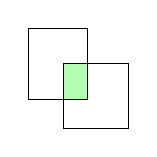
\begin{tikzpicture}[scale=0.75]
		\draw (0,0) rectangle (1,1.2);
		\draw (0.6,0.6) rectangle (1.7,-0.5);
		\draw[fill=green!30] (0.6,0.6) rectangle (1,0);
		\end{tikzpicture}
		\item \abs 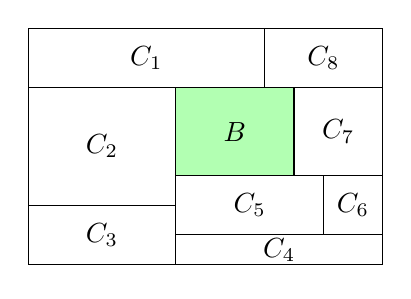
\begin{tikzpicture}[scale=0.75]
		\draw (0,0) rectangle (6,4);
		\draw[fill=green!30] (2.5,1.5) rectangle (4.5,3);		
		\draw (3.5, 2.25) node {$B$};
		\draw (0,4) rectangle (4,3);		
		\draw (2, 3.5) node {$C_1$};
		\draw (0,3) rectangle (2.5,1);
		\draw (1.25, 2) node {$C_2$};
		\draw (2.5,1.5) rectangle (5,0.5);
		\draw (3.75, 1) node {$C_5$};s
		\draw (4,4) rectangle (6,3);
		\draw (5, 3.5) node {$C_8$};
		\draw (4.5,3) rectangle (6,1.5);
		\draw (5.25, 2.25) node {$C_7$};
		\draw (0,1) rectangle (2.5,0);
		\draw (1.25, 0.5) node {$C_3$};
		\draw (2.5,0) rectangle (6,0.5);
		\draw (4.25, 0.25) node {$C_4$};
		\draw (5,1.5) rectangle (6,0.5);
		\draw (5.5, 1) node {$C_6$};
		\end{tikzpicture}
	\end{enumerate}
	Nat\"urlich kann man das formell sauber hinschreiben, das gibt uns aber keinen Verst\"andnis Mehrwehrt.
\end{beispiel1}
Aus der zweiten Eigenschaft eines Semirings kann man durch Induktion sofort Abgeschlossenheit bez\"uglich endlich vielen Schnitten zeigen. Probiert's einfach aus, ist zu einfach als \"Ubungsaufgabe. Auch die letzte Eigenschaft kann man verallgemeinern. Bei Quadern ist das anschaulich klar: Wenn man aus einem Quader endlich viele Quader entfernt, bleibt eine disjunkte Vereinigung von Quadern \"ubrig. Mit Induktion kriegen wir das auch f\"ur allgemeine Semiringe hin: 
\begin{lemma}\label{Skriptschreiberlemma} \link{https://www.youtube.com/watch?v=eLWjBR34aC0&list=PLy5qRKPWp6SBwfc1kn-b66cWc84cOgvqZ&index=4&t=4446s} \textbf{[Eine kleine Indexschlacht]}
	Es gilt in einem Semiring auch $\text{(iii)}'$: Sind $B_1,...,B_r,A\in \mathcal S$ mit  $B_1,B_2,...,B_r$ paarweise disjunkt, so existieren $C_1,...,C_n \in \cS$ paarweise disjunkt mit \[A \backslash (B_1 \cupdot ... \cupdot B_r) = \bigcupdot\limits_{k=1}^{n} C_k.\]
\end{lemma}

\begin{proof}
	Vollständige Induktion bezüglich $r$. \begin{itemize}
		\item [IA:] Für $A \backslash B_1$ folgt das direkt aus der Definition des Seminrings.
		\item [IV:] Die Behauptung gelte für ein beliebiges aber festes $r \in \N$.
		\item [IS:] Seien nun $B_1,B_2,...,B_{r+1} \in \mathcal S$ paarweise disjunkt. Nach Induktionsvoraussetzung und Rechenregeln mit Schnitten von Mengen gilt mit Umklammern von Schnitten und Vereinigungen
		\begin{align*}
		A \backslash \bigcupdot\limits_{i = 1}^{r+1} B_i &= A\cap  \bigcap_{i=1}^{r+1} B_i^C\\
		 &= \Big(A\backslash \bigcupdot_{i=1}^r B_i\Big) \cap B_{r+1}^C\\
		 & \overset{\text{IV}}{=} \Big(\bigcupdot\limits_{k = 1}^{m_r}  C_{r,k}\Big) \cap  B_{r + 1}^C
		 =\bigcupdot\limits_{k = 1}^{m_r} [C_{r,k} \backslash B_{r + 1}].
		\end{align*}
		Nun existieren für alle $1 \leq k \leq m_r$ jeweils endlich viele paarweise disjunkte Mengen $C_{r,k,1},...,C_{r,k,l_{r,k}} \in \cS$, mit 
		\[ C_{r,k} \backslash B_{r + 1} = \bigcupdot\limits_{m = 1}^{l_{r,k}} C_{r,k,m}. \]
		Also gilt \[
		A \backslash \bigcup\limits_{i = 1}^{r+1} B_i = \bigcupdot\limits_{k = 1}^{m_r} \bigcupdot\limits_{m = 1}^{l_{r,k}} C_{r,k,m}. \]
		Da die endlich vielen Mengen $C_{r,k,m}$ paarweise disjunkt sind, haben wir die gewünschte Darstellung f\"ur $A \backslash (B_1 \cupdot ... \cupdot B_{r+1})$ gefunden.
	\end{itemize}
\end{proof}
%Weiter geht es mit einer Versch\"arfung von Semiringen:
%\begin{deff}\label{Ring}
%	$\cR \in \cP(\Omega)$ heißt Ring, falls
%	\begin{enumerate}[label=(\roman*)]
%		\item $\emptyset \in \cR$
%		\item $A, B \in \cR \Rightarrow A \backslash B \in \cR$
%		\item $A,B \in \cR \Rightarrow A \cup B \in \cR$
%	\end{enumerate}
%\end{deff}

%\begin{bem1} \abs
%	\begin{enumerate}[label=(\roman*)]
%		\item $A^C$ ist nicht unbedingt in $\cR$, denn $\Omega \in \cR$ muss nicht gelten. Das sieht %harmlos aus, macht uns das Leben aber deutlich schwieriger.
%		\item Mit vollständiger Induktion sind auch endliche Vereinigungen wieder in $\cR$.
%	\end{enumerate}
%\end{bem1}



\marginpar{\textcolor{red}{Vorlesung 4}}


%\begin{bem}
%	$\cR$ Ring $\Rightarrow \cR$ Semiring. 
%\end{bem}

%\begin{proof}\abs
%	\begin{enumerate}[label=(\roman*)]
%		\item $\checkmark$
%		\item Folgt sofort aus der Beobachtung $A \cap B = A \backslash (A \backslash B)$.
%		\item Folgt sofort mit $n=1$, denn $A \backslash B \in \cR$.
%	\end{enumerate}
%\end{proof}

%Um ein besseres Gef\"uhl f\"ur die Definitionen zu bekommen, zeigen wir, dass die Menge der altbekannten disjunkten Vereinigungen von Quadern ein Ring bildet. Allgemeiner geht das f\"ur beliebige Semiringe:

%\begin{bem}
%	Ist $\cS$ ein Semiring, so ist die Menge aller endlicher disjunkter Vereinigungen
%	\[ \cR := \left\{ \bigcupdot\limits_{i = 1}^{n} A_i \! : n \in \N, \: A_1,...,A_n \in \cS \right\} \]
%	der kleinste Ring, der $\cS$ enth\"alt.
	% die Formulierung im Skript von Gärtner finde ich persönlich hübscher: "Man kann auf natürliche Weise aus jedem Semiring S einen Ring R konstruieren."
%\end{bem}

%\begin{proof}
%	Dass $\cR$ der \textit{kleinste} Ring ist, ist klar (es gilt $\cS \subseteq \cR$ mit $n=1$ und damit m\"ussen aufgrund der Eigenschaft eines Rings alle endlichen Vereinigungen wieder enthalten sein). Wir m\"ussen also noch zeigen, dass $\cR$ tats\"achlich ein Ring ist. Checken wir also die Eigenschaften:
%	\begin{enumerate}[label=(\roman*)]
%		\item $\checkmark$
%		\item \label{A,B} Seien dazu $A, B\in \cR$, also
%		\begin{gather*}
%			A = \bigcupdot\limits_{i=1}^{n} A_i\quad \text{ und }\quad  B = \bigcupdot\limits_{j=1}^{m} B_j.
%		\end{gather*}
%		Dann gilt
%			\begin{gather*}
%			A \backslash B = \bigcupdot\limits_{i=1}^{n} \underbrace{\Big( A_i \backslash \bigcupdot\limits_{j=1}^{m} \underbrace{(A_i \cap B_i)}_{\substack{\in \cS \text{, weil }\\ \cS \: \cap \text{-stabil}}}\Big)}_{\overset{\text{\ref{Skriptschreiberlemma}}}{=} \bigcupdot \limits_{k=1}^{r} C_{i,k}}\\
%			= \bigcupdot \limits_{i=1}^{n} \bigcupdot \limits_{k=1}^{r_i} C_{i,k}.
%		\end{gather*}
%		\item Seien $A,B$ wie in \ref{A,B}, so gilt $ A \cup B = \underbrace{(A\backslash B)}_{\in \cR} \cupdot \underbrace{B}_{\in \cR} \overset{\text{Def.}}{\in} \cR$ weil eine disjunkte Vereinigungen disjunkter Mengen in $\mathcal S$ wieder eine disjunkte Vereinigung von Mengen in $\mathcal S$ ist.
%	\end{enumerate}
%\end{proof}

%\begin{deff}
%	$\cA \subseteq \cP(\Omega)$ heißt Algebra, falls $\cA$ ein Ring ist und $\Omega \in \cA$.
%\end{deff}
%Die Definition einer Algebra ist \"aquivalent zur Forderung
%	\begin{enumerate}[label=(\roman*)]
%		\item $\emptyset \in \cA$,
%		\item $A \in \cA \Rightarrow A^C \in \cA$,
%		\item $A_1,...,A_n \in \cA \Rightarrow \bigcup\limits_{i = 1}^{n} A_i \in \cA$,
%	\end{enumerate}
%weil $\Omega\backslash A=A^C$.
%\begin{deff}
%	$\cR \subseteq \cP(\Omega)$ heißt $\sigma$-Ring, falls (iii) in der Definition des Rings durch 
%	\begin{align*}
%		A_1,A_2,... \in \cR \Rightarrow \bigcup\limits_{i = 1}^{\infty} A_i \in \cR 
%	\end{align*}
%	ersetzt wird. Das $\sigma$ steht also wieder für \enquote{abzählbar viele}.
	% Wir haben bei der ersten Definition des Maßes schon so nen ähnlichen Satz; ist nicht schlimm, aber könnte man evtl. auch in nur einen Satz zusammenführen.
%\end{deff}
%	Ein $\sigma$-Ring $\cR$ mit $\Omega \in \cR$ ist also nichts anderes als eine $\sigma$-Algebra.

Es kommen jetzt ein paar schmerzhafte Vorbereitungen f\"ur den wichtigsten Satz dieses Abschnitts, den Fortsetztungssatz von Carath\'eodory. Wir werden zun\"achst zeigen, dass die Monotonie und Subadditivit\"at (siehe Lemma \ref{monsub}) auch f\"ur \glqq Ma\ss e\grqq{} auf Semiringen gilt. Warum steht hier Ma\ss{} in Anf\"uhrungsstrichen? Per Definition ist ein Ma\ss{} immer auf einer $\sigma$-Algebra definiert, der Begriff macht also auf Semiringen gar keinen Sinn. Die genaue Aussage ist also, dass eine Mengenfunktion auf Semiringen mit Eigenschaften die einem Ma\ss{} \"ahneln, ebenfalls Monotonie und Subadditivit\"at erf\"ullen. 
\begin{lemma}\label{Rechenregeln} \link{https://www.youtube.com/watch?v=P2eNjbbLRa8&list=PLy5qRKPWp6SBwfc1kn-b66cWc84cOgvqZ&index=5&t=275s}\textbf{[Eine ziemlich gro\ss e Indexschlacht]}
	Sei $\cS$ ein Semiring und $\mu \! : \mathcal S \rightarrow [0, \infty] $ eine Mengenfunktion mit
	\begin{itemize}
		\item $\mu(\emptyset) = 0$
		\item $\mu$ ist \textbf{$\sigma$-additiv} (d.h. sind $A_1, A_2, ... \in S$ paarweise disjunkt mit $A:=\bigcupdot_{k=1}^\infty A_k\in \mathcal S$, so gilt $\mu(A)=\sum_{k=1}^\infty \mu(A_k)$).
	\end{itemize}
	Dann gilt
	\begin{enumerate}[label=(\roman*)]
		\item \label{MonotQuasiMass} Monotonie: $\mu(A) \leq \mu(B)$ für alle $A,B \in \cS$ mit $ A \subseteq B$.
		\item  \glqq \textbf{Subadditivit\"at}\grqq: Sind $A,A_1,A_2,... \in \cS $ und $A\subseteq \bigcup\limits_{k=1}^{\infty} A_k$, so gilt $ \mu(A) \leq \sum\limits_{k = 1}^{\infty} \mu(A_k).$
	\end{enumerate}
\end{lemma}
Man beachte, dass die Eigenschaften der $\sigma$-Additivit\"at etwas komisch sind. Da wir nicht fordern, dass Semiringe abgeschlossen bez\"uglich Vereinigungen sind (sie sind es auch meistens nicht, man denke nur an den Semiring der Quader), muss immer gefordert werden, dass die Vereinigungen wieder in $\cS$ liegen. Sonst w\"are $\mu(A)$ schlie\ss lich gar nicht definiert! Auch zu beachten ist, dass Vereinigungen und Komplemente nicht automatisch in $\mathcal S$ liegen. Daher sind einfache Eigenschaften f\"ur Ma\ss e auf $\sigma$-Algebren, nicht so einfach f\"ur Mengenfunktionen auf Semiringen.

\begin{proof}\abs
	\begin{enumerate}[label=(\roman*)]
		\item Es gibt wegen der Eigenschaften eines Semirings Mengen $C_1,...,C_m \in \cS$ mit \[B \backslash A = \bigcupdot\limits_{k=1}^m C_k.\] Damit gilt wegen der geforderten Additivit\"at von $\mu$
		\begin{align*}
		\mu(B) &= \mu(A \cupdot (B \backslash A)) = \mu(A \cupdot C_1 \cupdot ... \cupdot C_m) = \mu(A) + \mu(C_1) + ... + \mu(C_m)
		\geq \mu(A).
		\end{align*} 
		\item Erst machen wir (wie immer wieder!) die $A_n$ disjunkt:
		\begin{align*}
			A'_1 &:= A_1,\\
			A_2' &:= A_2 \backslash A_1',\\
			A_n' &:= A_n \backslash (A_1' \cupdot ... \cupdot A_{n-1}' ), \quad n \geq 3.
		\end{align*}
		\textit{Beachte:} Die $A'_{n}$ müssen nicht in in $\cS$ sein. Weil die $A'_{n}$ die Form $A_n \backslash ...$ haben, gibt es wegen Lemma \ref{Skriptschreiberlemma} allerdings paarweise disjunkte $C_{n,j} \in \cS$ mit 
		\begin{equation}\label{C_ns}
			A_{n}' = \bigcupdot\limits_{j=1}^{l_n} C_{n,j}
		\end{equation}
		für alle $n \in \N$. Darum gibt es wegen Lemma \ref{Skriptschreiberlemma} Mengen $D_{n,k} \in \cS$ mit
		\begin{equation}\label{D_nks}
			A_n \backslash A_{n}' = \bigcupdot\limits_{k = 1}^{m_n} D_{n,k}.
		\end{equation}
		Damit gelten
		\begin{itemize}
			\item 
			\begin{equation*}
				A = \bigcupdot\limits_{n=1}^{\infty} A'_{n} \cap A = \bigcupdot\limits_{n=1}^{\infty} \bigcupdot\limits_{j=1}^{l_n} A \cap C_{n,j}
			\end{equation*}
			weil $A\subseteq \bigcup\limits_{n=1}^{\infty} A_{n}= \bigcupdot\limits_{n=1}^{\infty} A_{n}'$ angenommen wurde,
			\item 
			\begin{gather*}
				A_n = A'_{n} \cupdot (A_n \backslash A'_{n}) \underset{\eqref{D_nks}}{\overset{\eqref{C_ns}}{=}} \bigcupdot\limits_{j=1}^{l_n} C_{n,j} \cupdot \bigcupdot\limits_{n = 1}^{m_n} D_{n,k}.
			\end{gather*}
		\end{itemize}
	Alles zusammen ergibt die Subadditivit\"at:
	\begin{align*}
		\mu(A) &= \mu\Big(\bigcupdot\limits_{n=1}^{\infty} \bigcupdot\limits_{j=1}^{l_n} \underbrace{A \cap C_{n,j}}_{\substack{\in \cS \text{, weil }\mathcal S\\ \cap \text{-stabil}}}\Big) \\
		\overset{\sigma \text{-add.}}&{=} \sum\limits_{n=1}^{\infty} \sum\limits_{j=1}^{l_n} \mu(A \cap C_{n,j}) \\ 
		\overset{\text{Monotonie}}&{\leq} \sum\limits_{n=1}^{\infty} \sum\limits_{j=1}^{l_n} \mu(C_{n,j}) \\
		\overset{\mu \geq 0}&{\leq} \sum\limits_{n=1}^{\infty} \Big( \sum\limits_{j=1}^{l_n} \mu(C_{n,j}) + \sum\limits_{k=1}^{m_n} \mu(D_{n,k})\Big) \\ 
		\overset{\sigma \text{-add.}}&{=} \sum\limits_{n=1}^{\infty} \mu\Big(\bigcupdot\limits_{n=1}^{l_n} C_{n,j} \cupdot \bigcupdot\limits_{j=1}^{m_n} D_{n,k}\Big)\\
		& = \sum\limits_{n=1}^{\infty} \mu(A_n).
	\end{align*}
	\end{enumerate}
\end{proof}
\begin{deff} \link{https://www.youtube.com/watch?v=P2eNjbbLRa8&list=PLy5qRKPWp6SBwfc1kn-b66cWc84cOgvqZ&index=5&t=2204s}
	$\mu^{*} \! : \cP (\Omega) \rightarrow [0,\infty]$ heißt \textbf{äußeres Maß}, falls
	\begin{enumerate}[label=(\roman*)]
		\item $\mu^{*}(\emptyset) = 0$
		\item $A \subseteq B \subseteq \Omega\, \Rightarrow \, \mu^{*}(A) \leq \mu^{*}(B)$
		\item $A_1,A_2,... \subseteq \Omega \, \Rightarrow \, \mu^{*} \Big(\bigcup\limits_{k=1}^{\infty} A_k \Big) \leq \sum\limits_{k=1}^{\infty} \mu^{*}(A_k)$
	\end{enumerate}
\end{deff}
F\"ur den Moment bleibt es unklar, weshalb wir dieser abstrakten Definition den Namen \glqq \"au\ss eres Ma\ss\grqq{} geben. Das wird aber in dem Beweis des Carath\'eodory Fortsetzungssatzes klar werden. Das dort definierte \"au\ss ere Ma\ss{} hat eine klare Interterpretation.
\begin{deff}\link{https://www.youtube.com/watch?v=P2eNjbbLRa8&list=PLy5qRKPWp6SBwfc1kn-b66cWc84cOgvqZ&index=5&t=2376s}
	Sei $\mu^{*}$ ein äußeres Maß auf $\Omega$. Dann heißt $A \subseteq \Omega$ \textbf{$\mu^{*}$-messbare Menge}, falls für alle $Z \subseteq \Omega$ \[ \mu^{*}(Z) = \mu^{*}(Z\cap A) + \mu^{*}(Z \cap A^C) \] gilt. Die Menge der $\mu^{*}$-messbaren Mengen heißt $\cA_{\mu^{*}}$.
\end{deff}

\begin{prop}
\link{https://www.youtube.com/watch?v=P2eNjbbLRa8&list=PLy5qRKPWp6SBwfc1kn-b66cWc84cOgvqZ&index=5&t=2556s} \abs 
	\begin{enumerate}[label=(\roman*)]		
		\item $\cA_{\mu^{*}}$ ist eine $\sigma$-Algebra.
		\item $\mu^{*}$ eingeschränkt auf $\cA_{\mu^{*}}$ ist ein Maß.
	\end{enumerate}
\end{prop}

\begin{proof}
	Wir zeigen nacheinander (a) $\cA_{\mu^{*}}$ ist eine $\sigma$-Algebra und (b) $\mu^{*}$ ist ein Maß auf $\cA_{\mu^{*}}$.\smallskip
	
	(a) Zu zeigen sind die definierenden Eigenschaften einer $\sigma$-Algebra:
		\begin{enumerate}[label=(\roman*)]
			\item F\"ur $Z \subseteq \Omega$ gilt 
			\begin{gather*}
			\mu^{*}(Z) = \mu^{*}(Z) + 0 = \mu^{*}(Z \cap \Omega) + \mu^{*}(Z \cap \underbrace{\Omega^C}_{= \emptyset}).
			\end{gather*}
			Damit ist $\Omega \in \cA_{\mu^{*}}$ gezeigt.
			\item Sei $A \in \cA_{\mu^{*}}$, dann erf\"ullt ($+$ kommutieren und $(A^C)^C=A$ nutzen) auch $A^C$ die definierende Eigenschaft von $\cA_{\mu^{*}}$. Also ist $\cA_{\mu^{*}}$ abgeschlossen unter Komplementbildung.
			\item Wir zeigen zun\"achst die Abgeschlossenheit bez\"uglich Vereinigungen von zwei Mengen. Seien also $A_1, A_2 \in \cA_{\mu^{*}}$. Sei $Z \subseteq \Omega$ beliebig, dann folgt mit $Z':= Z\cap (A_1\cup A_2)$
			\begin{align*}
			\mu^{*}(Z \cap (A_1 \cup A_2))
			\overset{A_1 \in \cA_{\mu^{*}}}&{=} \mu^*(Z\cap(A_1\cup A_2)\cap A_1)+\mu^*(Z\cap(A_1\cup A_2)\cap A_1^C)\\
			&= \mu^{*}(Z \cap A_1) + \mu^{*}(Z \cap A_2 \cap A_1^C).
			\end{align*}
			Folglich gilt auch
			\begin{align*}
			&\quad \mu^{*}(Z \cap (A_1 \cup A_2)) + \mu^{*}(Z \cap (A_1 \cup A_2)^C)\\
			&= \mu^{*}(Z \cap A_1) + \mu^{*}(Z \cap A_2 \cap A_1^C) + \mu^{*}(Z \cap (A_1 \cup A_2)^C)&\\
			&= \mu^{*}(Z \cap A_1) + \mu^{*}(\underbrace{Z \cap A_1^C}_{=: Z''} \cap A_2) + \mu^{*}(\underbrace{Z \cap A_1^C}_{=: Z''} \cap A_2^C)&\\
			\overset{A_2 \in \cA_{\mu^{*}}}&{=} \mu^{*}(Z \cap A_1) + \mu^{*}(Z \cap A_1^C)\\\overset{A_1 \in \cA_{\mu^{*}}}&{=} \mu^{*}(Z)
			\end{align*}
			und damit ist $A_1\cup A_2 \in \cA_{\mu^{*}}$.
		\item Per Induktion folgt aus (iii) die Abgeschlossenheit bez\"uglich Vereinigungen endlich vieler Mengen.
		\item Es fehlt jetzt noch die Abgeschlossenheit bez\"uglich abz\"ahlbar unendlicher Vereinigungen.
 Seien also $A_1,A_2,...\in \cA_{\mu^{*}}$, zu zeigen ist $\bigcup\limits_{n=1}^{\infty} A_n \in \cA_{\mu^{*}}.$ Zuerst nutzen wir den schon bekannten Trick, der uns erlaubt, ohne Einschr\"ankung der Allgemeinheit anzunehmen, dass die Mengen diskjunkt sind. Dazu definieren wir die paarweise disjunkten Mengen
	\begin{align*}
		A_1'=A_1, \quad A_2'=A_2\backslash A_1',\quad \text{ und }\quad A_n'= A_n \backslash (A_1' \cupdot ...\cupdot A_{n-1}'), \quad n \geq 3,
	\end{align*}
	und beachten, dass damit $\bigcup\limits_{n=1}^{\infty} A_n = \bigcupdot\limits_{n=1}^{\infty} A_n'$ gilt. Wenn also die Vereinigung der disjunkten $A_n'$ wieder in $\mathcal A_{\mu^*}$ ist, ist auch die Vereinigung \"uber die $A_n$ in $\mathcal A_{\mu^*}$. Es reicht also die Aussage f\"ur disjunkte Mengen zu beweisen. Damit die Rechnungen lesbarer bleiben, nehmen wir also ohne Beschr\"ankung der Allgemeinheit an, dass die Mengen $A_1, A_2, ...$ paarweise disjunkt sind, so sparen wir uns die $'$ in den Gleichungen. Aufgrund der Definition von $\mathcal A_{\mu^*}$ w\"ahlen wir ein $Z\subseteq \Omega$ beliebig. Wir zeigen erstmal induktiv 
	\begin{equation}\label{IndVor}
		\mu^{*}(Z)= \sum\limits_{k=1}^{n} \mu^{*}(Z \cap A_k) + \mu^{*}\Big(Z \cap \bigcap\limits_{k=1}^{n} A_k^C \Big),\quad \forall n \in \N.
	\end{equation}
	\begin{itemize}
		\item [IA:] Für $n=1$ gilt die Behauptung, weil $A_1 \in \cA_{\mu^{*}}$.
		\item [IV:] Es gelte \eqref{IndVor} für ein \underline{beliebiges, aber festes} $n \in \N$.
		\item [IS:] Eine kleine Runde Kampfrechnen mit Mengen. Weil nach Annahme $A_{n+1} \in \cA_{\mu^{*}}$ und die $A_n$ paarweise disjunkt sind, gilt
		\begin{align*}
			\mu^{*}\Big(Z \cap \bigcap\limits_{k=1}^{n} A_k^C \Big)
			&= \mu^{*}\Big(Z \cap \bigcap\limits_{k=1}^{n} A_k^C \cap A_{n+1} \Big) + \mu^{*}\Big(Z \cap \bigcap\limits_{k=1}^{n} A_k^C \cap A_{n+1}^C \Big)\\
			 &= \mu^{*}(Z \cap A_{n+1})+ \mu^{*}\Big(Z \cap \bigcap\limits_{k=1}^{n + 1} A_k^C \Big).
		\end{align*}
		Einsetzen in die Induktionsvoraussetzung gibt
		\begin{align*}
			\mu^{*}(Z) & = \sum\limits_{k = 1}^{n + 1} \mu^{*}(Z \cap A_k) + \mu^{*}\Big(Z \cap \bigcap\limits_{k=1}^{n + 1} A_k^C \Big).
		\end{align*}
		Damit ist der Induktionsschritt gezeigt.
	\end{itemize}
	Zur\"uck zur Vereinigung: Wegen der angenommenen Monotonie von $\mu^*$ folgt aus \eqref{IndVor}  \[ \mu^{*}(Z) \geq \sum\limits_{k=1}^{n} \mu^{*}(Z \cap A_k) + \mu^{*}\Big(Z \cap \bigcap\limits_{k = 1}^{\infty} A_k^C\Big), \quad \forall n \in \N. \]
		Mit $n \to \infty$ folgt (Monotonie von Grenzwertbildung aus Analysis 1)
		\begin{align}\label{ab}
		\begin{split}
			\mu^{*}(Z) &\geq \sum\limits_{k=1}^{\infty} \mu^{*}(Z \cap A_k) + \mu^{*}\Big(Z \cap \bigcap\limits_{k = 1}^{\infty} A_k^C\Big)\\ 
			&\geq \mu^{*} \Big(\bigcup\limits_{k = 1}^{\infty} A_k \cap Z \Big) + \mu^{*}\Big(Z \cap \Big(\bigcup\limits_{k = 1}^{\infty} A_k\Big)^C\Big)\\
			&\geq  \mu^{*}\Big(\Big(Z \cap \bigcup\limits_{k = 1}^{\infty} A_k\Big) \cup \Big(Z\cap \Big(\bigcup\limits_{k = 1}^{\infty} A_k\Big)^C\Big)\Big)\\
			& = \mu^{*}\Big(Z \cap \underbrace{\Big(\bigcup\limits_{k= 1}^{\infty} A_k\cup \Big(\bigcup\limits_{k= 1}^{\infty} A_k\Big)^C\Big)}_{\Omega}\Big) = \mu^{*}(Z).
		\end{split}
		\end{align}
		F\"ur die letzten beiden Ungleichungen haben wir die angenommene Subadditivit\"at (Ungleichung andersrum als \"ublich) genutzt. 
	Weil die linke und rechte Seite der Kette von Ungleichungen identisch sind, sind die Ungleichungen alles Gleichungen, also gilt \[ \mu^{*}(Z) = \mu^{*}\Big(Z \cap \bigcup\limits_{k=1}^{\infty} A_k\Big) + \mu^{*}\Big(Z \cap \Big(\bigcup\limits_{k=1}^{\infty} A_k\Big)^C\Big).  \] Weil $Z$ beliebig war, ist damit \[ \bigcup\limits_{k=1}^{\infty} A_k \in \cA_{\mu^{*}} \] aufgrund der Definition von $\mathcal A_{\mu^*}$.	Damit ist die Abgeschlossenheit bez\"uglich abz\"ahlbarer Vereinigungen gezeigt und folglich ist $\cA_{\mu^{*}}$ eine $\sigma$-Algebra. 
		\end{enumerate}

	
	(b) Aufgrund der Gleichheiten in \eqref{ab} gilt auch
	 \[ \mu^{*}(Z) = \sum\limits_{k = 1}^{\infty} \mu^{*}(Z \cap A_k) + \mu^{*}\Big(Z \cap \bigcap\limits_{k = 1}^{\infty} A_k^C\Big). \] 
	Wählen wir  $	Z = \bigcup\limits_{k = 1}^{\infty} A_k$, so gilt wegen $\mu(\emptyset)=0$
	\begin{align*}
		 \mu^{*}\Big(\bigcup\limits_{k = 1}^{\infty} A_k\Big)=\sum\limits_{k = 1}^{\infty} \mu^{*}(A_k) + 0
	\end{align*}
	und das ist gerade die $\sigma$-Additivit\"at von $\mu^*$. Also ist $\mu^*$ auch ein Ma\ss{} auf der $\sigma$-Algebra $\mathcal A_{\mu^*}$.
\end{proof}
\marginpar{\textcolor{red}{Vorlesung 5}}
Kommen wir endlich zum H\"ohepunkt der ersten Wochen. Nach dem Beweis sind wir auch endlich mitten in der Stochastik angelangt! Der Beweis enth\"alt tats\"achlich viele Informationen. Insbesondere wird klar, wo der Begriff \"au\ss eres Ma\ss{} herkommt.
\begin{satz} \label{KarlTheodor} \link{https://www.youtube.com/watch?v=nlUyBvwBkhE&list=PLy5qRKPWp6SBwfc1kn-b66cWc84cOgvqZ&index=6&t=164s} \textbf{[Fortsetzungssatz von Carathéodory]}
	Sei $\cS$ ein Semiring und $\mu \! : \mathcal S \rightarrow [0, \infty] $ eine Mengenfunktion mit
	\begin{itemize}
		\item $\mu(\emptyset) = 0$,
		\item $\mu$ ist \textbf{$\sigma$-additiv} (d.h. sind $A_1, A_2, ... \in S$ paarweise disjunkt mit $A:=\bigcupdot_{k=1}^\infty A_k\in \mathcal S$, so gilt $\mu(A)=\sum_{k=1}^\infty \mu(A_k)$).
	\end{itemize}
	Dann existiert ein Maß $\bar{\mu}$ auf $\sigma(\mathcal S)$ mit $\mu(A) = \bar{\mu}(A)$ für alle $A \in \cS$.
\end{satz}
Man sagt, dass die Mengenfunktion $\mu$ von $\cS$ nach $\sigma(\cS)$ \glqq fortgesetzt\grqq{} wird.

\begin{proof}
	Für $A \in \cP(\Omega)$ definieren wir \[ \mu^{*}(A) = \inf\Big\{ \sum\limits_{k=1}^{\infty} \mu(A_k) \! : A_1,A_2,... \in \cS \text{ mit } A \subseteq \bigcup\limits_{k = 1}^{\infty} A_k \Big\}. \]
	Beachte: Weil per Definition (Analysis 1) $\inf \emptyset=+\infty$ gilt, ist $\mu*(A)$ auch definiert, wenn man $A$ nicht durch Mengen aus $\mathcal S$ \"uberdecken kann. \smallskip
	
	Wir zeigen nun nacheinander (a) $\mu^*$ ist ein \"au\ss eres Ma\ss{}, (b) $\cS \subseteq \mathcal A_{\mu^*}$ und (c) $\mu^*(A)=\mu(A)$ f\"ur alle $A\in \cS$. Der Beweis ist dann vollendet, weil nach dem vorherigen Satz $\mathcal A_{\mu^*}$ eine $\sigma$-Algebra ist und $\mu^*$ ein Ma\ss{} auf $\mathcal A_{\mu^*}$ ist. Wegen (b) gilt $\sigma(S)\subseteq \mathcal A_{\mu^*}$, weil die kleinste $\sigma$-Algebra die $\cS$ enth\"alt, auch Teilmenge von allen $\sigma$-Algebras ist, die $\cS$ enthalten. Damit ist auch die Einschr\"ankung von $\mu^*$ auf $\sigma(S)$ ein Ma\ss{} (wir setzen dann $\bar{\mu} := \mu^{*}_{|{\sigma(\cS)}}$) und wegen (c) ist $\bar\mu$ eine Fortsetzung von $\mu$.
\begin{enumerate}[label=(\alph*)]
\item	Wir checken die definierenden Eigenschaften eines \"au\ss eren Ma\ss es:
	\begin{itemize}
		\item[(i)] $\mu^{*}(\emptyset) = 0$ ist klar, weil $\emptyset \in \mathcal S$ und $\mu(\emptyset)=0$.
		\item[(ii)] Monotonie folgt direkt aus der Definition.
		\item[(iii)] Nun zur Subadditivität. Seien dazu $A_1,A_2,... \in \mathcal P(\Omega)$ und $A = \bigcup\limits_{k = 1}^{\infty} A_k.$ Wir k\"onnen annehmen, dass $ \: \mu^{*}(A_k) < \infty$ f\"ur alle $k\in\N$ gilt (sonst gilt die Ungleichung sowieso). Sei nun $\varepsilon > 0$ beliebig. Für jedes $k \in \N$ existiert qua Definition (Infimum ist die gr\"o\ss te untere Schranke) eine Folge von Mengen $A_{k,1},A_{k,2},... \in \cS$ mit
		\begin{align*}
			A_k \subseteq \bigcup\limits_{j=1}^{\infty} A_{k,j} \quad \text{ und }\quad \sum\limits_{j=1}^{\infty} \mu(A_{k,j}) \leq \mu^{*}(A_k) + \frac{\varepsilon}{2^k}.			\end{align*}
		Wem das nicht klar ist, der schaue bitte in den Analysis 1 Mitschrieb! Weil \[A \overset{\text{Def.}}{=} \bigcup\limits_{k = 1}^{\infty} A_k \subseteq \bigcup\limits_{k = 1}^{\infty} \bigcup\limits_{j=1}^{\infty} A_{k,j} \] gilt, folgt (das Infimum einer Menge ist kleiner gleich jedem Element der Menge) 
		\begin{gather*}
			\mu^{*}(A) \underset{\text{als } \inf}{\overset{\text{Def. } \mu^{*}}{\leq}} \sum\limits_{k= 1}^{\infty} \sum\limits_{j= 1}^{\infty} \mu(A_{k,j}) \leq \sum\limits_{k = 1}^{\infty} \Big( \mu^{*}(A_k) + \frac{\varepsilon}{2^k} \Big) = \sum\limits_{k = 1}^{\infty} \mu^{*}(A_k) + \underbrace{\sum_{k=1}^\infty \frac{\varepsilon}{2^k}}_{\varepsilon}.
		\end{gather*}
		Weil $\varepsilon$ beliebig gew\"ahlt wurde, gilt damit die Subadditivit\"at von $\mu^*$. An dieser Stelle eine kleine Anmerkung: Eine \"Uberdeckung durch eine abz\"ahlbare Vereinigung von abz\"ahlbaren Vereinigungen ist gleichbedeutend zu nur einer abz\"ahlbaren Vereinigung. Das Stichwort ist Cantors Diagonalverfahren, siehe Analysis 1 (oder irgendeine andere Quelle). Wir k\"onnen Paare von nat\"urlichen Zahlen auf verschiedenen Weisen z\"ahlen: Zeilenweise, Spaltenweise, oder wie eine Schlange im Diagonalverfahren.
	\end{itemize}
	\item 	
		Wir zeigen $\cS \subseteq \cA_{\mu^{*}}$. Dazu m\"ussen wir $$\mu^{*}(Z) = \mu^{*}(Z \cap S) + \mu^{*}(Z \cap S^C),\quad \text{für alle }Z \subseteq \Omega, S \in \cS,$$ nachrechnen.
		
		\enquote{$\leq$}: $\mu^{*}(Z) = \mu^{*}((Z \cap S )\cupdot (Z \cap S^C)) \leq \mu^{*}(Z \cap S) + \mu^{*}(Z \cap S^C)$ gilt aufgrund der gezeigten Subadditivit\"at von $\mu^*$.
		
		\enquote{$\geq$}: Seien $A_1,A_2,... \subseteq \cS$ mit $Z \subseteq \bigcup\limits_{k= 1}^{\infty} A_k.$ Weil $\cS$ ein Semiring ist, existieren $C_{k,1},..., C_{k,m_k} \in \cS$ mit \[ A_k \cap S^C = A_k \backslash S = \bigcupdot\limits_{j= 1}^{m_k} C_{k,j}. \]
		Es gelten 
			 \[ Z \cap S \subseteq \Big(\bigcup\limits_{k = 1}^{\infty} A_k\Big) \cap S = \bigcup\limits_{k = 1}^{\infty} \big( A_k \cap S \big) \]
			 sowie analog
			 \[ Z \cap S^C \subseteq  \Big(\bigcup\limits_{k = 1}^{\infty} A_k\Big) \cap S^C= \bigcup\limits_{k = 1}^{\infty} \big( A_k \cap S^C \big)=\bigcup\limits_{k = 1}^{\infty}\bigcupdot\limits_{j= 1}^{m_k} C_{k,j}. \]
		Mit den Definitionen folgt
		\begin{align*}
			\mu^{*} (Z \cap S) + \mu^{*} (Z \cap S^C) 
			&\leq \sum\limits_{k=1}^{\infty} \Big(\mu( A_k\cap S) +\sum\limits_{j=1}^{m_k} \mu(C_{k,j})\Big )\\
			\overset{\mu\,\sigma\text{-add.}}&{=} \sum\limits_{k=1}^{\infty} \mu \Big((A_k \cap S) \cupdot \bigcupdot\limits_{j=1}^{m_k} C_{k,j} \Big)\\
			& = \sum\limits_{k=1}^{\infty} \mu \big((A_k \cap S )\cupdot( A_k \cap S^C)\big)\\
			&=\sum_{k=1}^\infty \mu(A_k).
		\end{align*}
		Daraus folgt $\mu^{*}(Z \cap S) + \mu^{*}(Z \cap S^C) \leq \mu^{*}(Z)$, weil \[\mu^{*}(Z) = \inf\left\{ \sum\limits_{k=1}^{\infty} \mu(A_k) \! : A_1,A_2,... \in \cS \text{ mit } Z \subseteq \bigcup\limits_{k = 1}^{\infty} A_k \right\}.\] Somit ist \enquote{$\geq$} gezeigt.		
		Also ist jedes $S \in A_{\mu^{*}}$ und damit gilt $\cS \subseteq A_{\mu^{*}}$.
		
		\item Fehlt noch $\mu^{*}(A) = \mu(A)$ für alle $A \in \cS$. Im Prinzip ist das Lemma \ref{Rechenregeln}.\smallskip
		
		\enquote{$\leq$}: \[ \mu^{*}(A) = \inf\left\{ \sum\limits_{k=1}^{\infty} \mu(A_k) \! : A_1,A_2,... \in \cS \text{ mit } A \subseteq \bigcup\limits_{k = 1}^{\infty} A_k \right\} \leq \mu(A) \:  \]f\"ur alle $A\in \mathcal S$.
		
		\enquote{$\geq$}:  Ist $A \subseteq \bigcup\limits_{k=1}^{\infty} A_k$ f\"ur $A_1,A_2,... \in \cS$, 
		so gilt \[ \mu(A) \overset{\ref{Rechenregeln}}{\leq} \sum\limits_{k=1}^{\infty} \mu(A_k). \] Folglich gilt \[ \mu(A) \leq \inf\left\{ \sum\limits_{k=1}^{\infty} \mu(A_k) \! : A_1,A_2,... \in \cS \text{ mit } A \subseteq \bigcup\limits_{k = 1}^{\infty} A_k \right\} = \mu^{*}(A). \]		
		
	\end{enumerate}
\end{proof}
Wir fassen nun den Existenz- und den Eindeutigkeitssatz zusammen, das gibt folgendes zentrale Theorem:
\begin{satz}\label{ExistMasse} \link{https://www.youtube.com/watch?v=nlUyBvwBkhE&list=PLy5qRKPWp6SBwfc1kn-b66cWc84cOgvqZ&index=6&t=3820s} \textbf{[Existenz und Eindeutigkeit von Maßen] }
	Es sei $(\Omega, \cA)$ ein messbarer Raum, $\cE$ ein Semiring mit $\sigma(\cE) = \cA$ und $\mu \! : \cE \rightarrow [0,\infty]$ eine Mengenfunktion mit
	\begin{itemize}
		\item $\mu(\emptyset) = 0$
		\item $\mu$ ist $\sigma$-additiv
		\item es gibt eine Folge $E_1,E_2,... \in \cE$ mit $E_n \uparrow \Omega$ und $\mu(E_n) < \infty$ f\"ur alle $n\in\N$.
	\end{itemize}
	Dann existiert genau ein Maß $\bar{\mu}$ auf $\cA = \sigma(\cE)$, so dass $\bar{\mu}(A) = \mu(A)$ f\"ur alle $A\in \cE$.
\end{satz}

\begin{proof}
	Existenz folgt direkt aus \ref{KarlTheodor}, Eindeutigkeit folgt direkt aus Satz \ref{folg}.
\end{proof}
Merkt euch f\"ur immer folgendes, das hilft euch, die verschiedenen Konzepte einzuordnen:
\begin{center}
	\textbf{Existenz ist Carath\'eodory mit \"au\ss eren Ma\ss en, Eindeutigkeit folgt aus Dynkin-Systemen!}
\end{center}
Anschlie\ss end an die abstrakte Theorie wollen wir nun als Beispiel die Borel-$\sigma$-Algebra auf $\R$ diskutieren. Hier wird alles viel klarer werden und das ist gerade die Anwendung, die wir f\"ur die Stochastik brauchen.



\section[Das Beispiel f\"ur Wahrscheinlichkeitsma\ss e]{Das Beispiel - Wahrscheinlichkeitsmaße auf $\mathcal B(\R)$ aus Verteilungsfunktionen}\label{sec:VF}
Das Konzept von Verteilungsfunktionen von Wahrscheinlichkeitsma\ss en auf $\mathcal B(\R)$ ist euch bereits bei Dynkin-Systemen und in den \"Ubungen \"uber den Weg gelaufen. Definieren wir nun abstrakt, welche reellen Funktionen wir Verteilungsfunktionen nennen wollen:
\begin{deff}
\link{https://www.youtube.com/watch?v=nlUyBvwBkhE&list=PLy5qRKPWp6SBwfc1kn-b66cWc84cOgvqZ&index=6&t=4310s}
	$F \! : \mathbb{R} \rightarrow \mathbb{R}$ heißt \textbf{Verteilungsfunktion}, falls 
	\begin{enumerate}[label=(\roman*)]
		\item $0 \leq F(t) \leq 1$ f\"ur alle $t\in\R$,
		\item $F$ ist nicht fallend,
		\item $F$ ist rechtsstetig, \mbox{d. h.} $\lim\limits_{s \downarrow t} F(s) = F(t)$,
		\item $\lim\limits_{t \to \infty} F(t) = 1$ und $\lim\limits_{t \to - \infty} F(t) = 0$.
	\end{enumerate}
\end{deff}
Der Hauptsatz \"uber Wahrscheinlichkeitsma\ss e auf $\mathcal B(\R)$ ist nun folgender bijektiver Zusammenhang zu Verteilungsfunktionen:
\begin{satz}\label{EindVert}
\link{https://www.youtube.com/watch?v=nlUyBvwBkhE&list=PLy5qRKPWp6SBwfc1kn-b66cWc84cOgvqZ&index=6&t=4500s} \textbf{[Wahrscheinlichkeitsma\ss e aus Verteilungsfunktionen]}
	Für jede Vertei-lungsfunktion F gibt es \textbf{genau ein} Wahrscheinlichkeitsmaß $\mathbb{P}_F$ und $\cB(\mathbb{R})$ mit $$\mathbb{P}_F((-\infty,t]) = F(t), \quad t \in \mathbb R.$$ Man sagt dann, \enquote{$\mathbb{P}_F$ ist gemäß $F$ verteilt} oder \enquote{$\mathbb{P}_F$ hat Verteilung $F$} und schreibt $\mathbb{P}_F\sim F$.
\end{satz}

\begin{proof}
\textbf{Eindeutigkeit}: Das haben wir uns schon in Beispiel \ref{eindm} \"uberlegt.\smallskip

\textbf{Existenz}: Um den Fortsetzungssatz von Carath\'eodory zu nutzen, m\"ussen wir zun\"achst einen Semiring w\"ahlen, der die Borel-$\sigma$-Algebra erzeugt. Wir wissen bereits, dass alle m\"oglichen Arten von Intervallen $\mathcal B(\R)$ erzeugt, die meisten sind aber keine Semiringe. Wir nehmen $$\cS = \{ (a,b]: a\leq b \},$$ und stellen sofort fest (Eigenschaften checken), dass $\cS$ ein Semiring mit $\sigma(\cS) = \cB(\mathbb{R})$ ist. Als Mengenfunktion auf $\cS$ definieren wir $$\mu((a,b]): = F(b) - F(a),\quad a\leq b.$$ Weil $F$ nicht-fallend ist und $0\leq F\leq 1$ gilt, bildet $\mu$ nach $[0,1]$ ab. Checken wir als n\"achstes die Voraussetzungen vom Fortsetzungssatz:
	\begin{enumerate}[label=(\roman*)]
		\item $\mu(\emptyset) = \mu((a,a]) = F(a) -F(a) = 0$
		\item F\"ur die $\sigma$-Additivität von $\mu$ auf $\mathcal S$ seien $(a_n,b_n] \in \cS$ paarweise disjunkt mit \[
		\bigcupdot\limits_{k= 1}^{\infty} (a_k,b_k] \in \cS, \quad \text{ also } \bigcupdot \limits_{k = 1}^{\infty} (a_k,b_k] =: (a,b], \]
		f\"ur geeignete $a,b\in\R$. Als Anschauungsbeispiel haltet ihr am besten das konkrete Beispiel $(0,1] = \bigcupdot \limits_{k=1}^{\infty} (\frac{1}{k+1}, \frac{1}{k}]$ im Kopf. Um den Beweis besser zu verstehen, schauen wir uns erstmal den endlichen Fall an, d. h. \[ (a,b] = \bigcupdot\limits_{k=1}^{N} (a_k,b_k], \] f\"ur ein $N\in\N$ mit geordneten Intervallen $a=a_1<b_1= a_2<...<b_N=b$. Dann bekommen wir die $\sigma$-Additivit\"at sofort:
		\begin{gather*}
			\mu((a,b]) \overset{\text{Def.}}{=} F(b) - F(a) \overset{\text{Teleskop}}{=} \sum\limits_{k=1}^{N} (F(b_k) - F(a_k)) = \sum\limits_{k=1}^{N} \mu((a_k,b_k]),
		\end{gather*}
		wobei wir $F(a_k)=F(b_{k-1})$ genutzt haben.
		\marginpar{\textcolor{red}{Vorlesung 6}}
			Nun aber zurück zum allgemeinen Fall: Wir zeigen 
		\begin{align}\label{dd}
		 F(b) - F(a) = \sum\limits_{k=1}^{\infty} (F(b_k) - F(a_k)),
		 \end{align}
		  denn das ist gerade die $\sigma$-Additivit\"at
		\begin{align*}
			\mu\Big(\bigcupdot_{k=1}^\infty (a_k,b_k]\Big)=\sum_{k=1}^\infty \mu((a_k,b_k])
		\end{align*}		
		f\"ur $(a,b] = \bigcupdot\limits_{k = 1}^{\infty} (a_k,b_k]$.	F\"ur die Gleichheit \eqref{dd} zeigen wir beide Ungleichungen:
		\begin{itemize}
			\item [\enquote{$\geq$}:] Weil $F$ nicht-fallend ist, folgt \[ F(b) - F(a) \geq F(b_N)-F(a_1)\overset{\text{Teleskop}}{=} \sum\limits_{k=1}^{N} (F(b_k) - F(a_k))\] f\"ur alle $N\in\N$. 
			Wegen der Monotonie von Folgengrenzwerten gilt \[ F(b) - F(a) \geq \lim\limits_{N \to \infty} \sum\limits_{k=1}^{N} (F(b_k) - F(a_k)) = \sum\limits_{k=1}^{\infty} (F(b_k) - F(a_k)). \]
			\item [\enquote{$\leq$}:] Sei $\varepsilon > 0$ und seien $b_n<\tilde{b}_n$, so dass
			\begin{align}\label{ee}
			 	 0 \leq F(\tilde{b}_n) - F(b_n) < \frac{\varepsilon}{2^n}
			\end{align}	
			f\"ur alle $n\in\N$. Die $\tilde{b}_n$ existieren weil $F$ rechtsstetig ist (schreibt mal die Definition der Stetigkeit mit $\frac{\varepsilon}{2^n}$ statt $\varepsilon$ hin). Weil 
			\begin{align*}
				(a,b]=\bigcup\limits_{k = 1}^{\infty} (a_k,{b}_k]  \overset{b_k<\tilde b_k}{\subseteq} \bigcup\limits_{k = 1}^{\infty} (a_k,\tilde{b}_k)
			\end{align*}
				gilt, gilt auch \[ [a + \varepsilon, b] \subseteq \bigcup\limits_{k = 1}^{\infty} (a_k,\tilde b_k). \] Nach Heine-Borel ist $[a + \varepsilon, b]$ kompakt. Aufgrund der Definition der Kompaktheit reichen endlich viele $(a_k, \tilde{b}_k)$, um $[a + \varepsilon, b]$ zu überdecken. Also gibt es ein $N\in\N$ mit \[ [a + \varepsilon, b] \subseteq \bigcup\limits_{k = 1}^{N} (a_k, \tilde{b}_k). \] Daraus folgt dann
			\begin{align*}
				F(b) - F(a + \varepsilon) \overset{\text{F monoton}}&{\leq}  \sum\limits_{k=1}^{N} (F(\tilde{b}_k) - F(a_k))\\ 
				\overset{\eqref{ee}}&{\leq} \sum\limits_{k=1}^{\infty} (F(b_k) + \frac{\varepsilon}{2^k} - F(a_k)) = \sum\limits_{k=1}^{\infty} (F(b_k) - F(a_k)) + \varepsilon,
			\end{align*}
			wobei wir im letzten Schritt die geometrische Reihe $\sum_{k=1}^\infty \frac{1}{2^k}=1$ genutzt haben. Wegen der Rechtsstetigkeit von $F$ folgt damit
			\begin{align*}			
			  F(b) - F(a) &= \lim\limits_{\varepsilon \downarrow 0} (F(b) - F(a + \varepsilon))\\
			  & \leq \lim\limits_{\varepsilon \downarrow 0} \Big(\sum\limits_{k=1}^{\infty} (F(b_k) - F(a_k)) + \varepsilon\Big) = \sum\limits_{k=1}^{\infty} (F(b_k) - F(a_k)).
			\end{align*}			
		\end{itemize}
	Der Fortsetzungssatz impliziert nun die Existenz eines Maßes $\mathbb{P}_F$ auf $\cB(\mathbb{R})$ mit \[\mathbb{P}_F((a,b]) = \mu((a,b]) = F(b) - F(a),\quad a<b.\] Das Ma\ss{} ist nicht automatisch ein Wahrscheinlichkeitsma\ss, das folgt aber direkt aus der Stetigkeit von Ma\ss en und der Charakterisierung von $\mathbb P_F$ auf den Intervallen:
		\begin{align*}
			\mathbb{P}_F(\mathbb{R}) &= \mathbb{P}_F\Big(\bigcup\limits_{k = 1}^{\infty} (-k,k]\Big)\\
			 \overset{\text{Stet. Ma\ss e}}&{=} \lim\limits_{n \to \infty} \mathbb{P}_F((-n,n])\\
			\overset{\text{Def.}}&{=} \lim\limits_{n \to \infty} (F(n) - F(-n))\\
			& = \lim\limits_{n \to \infty} F(n) - \lim\limits_{n \to \infty} F(-n)=1.
		\end{align*}
		Achtung, das Argument werden wir jetzt immer wieder nutzen!\smallskip
		
		Ganz \"ahnlich zeigen wir den Zusammenhang von $F$ und $\mathbb P_F$ auf unendlichen Intervallen, wie im Satz behauptet wird:
		\begin{gather*}
			\mathbb{P}_F((-\infty,t]) = \mathbb{P}_F\Big(\bigcup\limits_{k = \left \lceil{|t|}\right \rceil }^{\infty} (-k,t]\Big) = \lim\limits_{k \to \infty} \mathbb{P}_F((-k,t])=F(t)-\lim_{k\to\infty} F(-k)=F(t),
		\end{gather*}
		wobei $\lceil |t|\rceil$ die obere Gau\ss klammer von $|t|$ ist, also $|t|$ aufgerundet.
	\end{enumerate}
\end{proof}

\begin{bem} \link{https://www.youtube.com/watch?v=8pGCVx1Z7fk&list=PLy5qRKPWp6SBwfc1kn-b66cWc84cOgvqZ&index=7&t=1912s}
	Es gibt ganz analog eine Definition für Verteilungsfunktionen auf dem $\mathbb{R}^d$, sogenannte \enquote{multivariate Verteilungsfunktionen} -- das machen wir später.
\end{bem}
Bevor wir zu Beispielen von Wahrscheinlichkeitsma\ss en auf $\mathcal B(\R)$ kommen, hier noch das zweite wichtige Ma\ss es auf der Borel-$\sigma$-Algebra - das Lebesgue-Ma\ss{} (Volumen) auf $\mathcal B(\R^d)$.
\begin{satz}
\link{https://www.youtube.com/watch?v=8pGCVx1Z7fk&list=PLy5qRKPWp6SBwfc1kn-b66cWc84cOgvqZ&index=7&t=1992s} \textbf{[Lebesgue-Ma\ss{} auf $\R^d$]}
	Es gibt ein eindeutiges Maß $\lambda$ auf $\mathcal B(\R^d)$ mit $\lambda(Q)=\text{ Volumen(Q)}$ für alle Quader $Q \subseteq \mathbb{R}^d$. $\lambda$ heißt Lebesgue-Maß auf $\R^d$ und ist ein unendliches Ma\ss.
\end{satz}

\begin{proof}
	Übung, ziemlich analog zum vorherigen Beweis. Wir checken die Voraussetzungen von Satz \ref{ExistMasse}, hier ist eine Skizze: Betrachte $$\cS := \big\{ (a_1,b_1]\times \dots \times (a_n,b_n] : a_1,\dots,a_d, b_1,\dots, b_d\in \R\big\},$$ $\cS$ ist ein Semiring.
		 $$\mu(Q) := \text{Volumen(Q)} = \prod\limits_{k=1}^{d}(b_k-a_k)$$ ist eine $\sigma$-additive Mengenfunktion auf $\cS$ (die $\sigma$-Additivit\"at zeigt man mit Kompaktheit im $\R^d$, genau wie im letzten Satz). Mit der Folge $E_n:=(-n,n]\times \dots (-n,n]\in \cS$ haben wir eine Folge mit endlichem Volumen, die gegen $\R^d$ w\"achst. Das ist die dritte Eigenschaft von Satz \ref{ExistMasse}, es gibt also eine eindeutige Fortsetzung von $\mu$ auf $\mathcal B(\R^d)$. Das Ma\ss{} nennen wir $\lambda$. Es fehlt noch, dass $\lambda$ ein unendliches Ma\ss{} ist. Aber auch das geht mit den Argumenten des vorherigen Beweises:
		 \begin{align*}
		 \lambda(\mathbb{R}^d) \overset{\text{Stet. Ma\ss e}}{=}\lim\limits_{n \to \infty}\lambda ((n,-n]\times ... \times (n,-n])  = \lim\limits_{n \to \infty} (2n)^d= \infty.
		 \end{align*}
\end{proof}
Meistens betrachten wir das Lebesguema\ss{} auf $\R$, das im Prinzip die \enquote{L\"ange} einer Menge misst, zumindest gilt das f\"ur Intervalle (oder disjunkte Vereinigungen von Intervallen). 
\begin{bem}
\link{https://www.youtube.com/watch?v=8pGCVx1Z7fk&list=PLy5qRKPWp6SBwfc1kn-b66cWc84cOgvqZ&index=7&t=2729s}
	Auf den \"Ubungsbl\"attern diskutieren wir das Lebesgue-Ma\ss{} auf Teilmengen vom $\R^d$, insbesondere auf Intervalle oder Quadern.  Beispielsweise sind dann die messbaren Mengen
	\begin{align*}
		\mathcal B([0,1]) :=\big\{ B\subseteq [0,1]: B\in \mathcal B(\R)\big\}=\sigma(\{[a,b]: 0\leq a<b\leq 1\})
	\end{align*}
	die Borel-messbaren Teilmengen von $[0,1]$ und $\lambda_{[0,1]}$ das eindeutige Ma\ss{} auf $\mathcal B([0,1])$ mit $\lambda_{[0,1]}(B)=\lambda(B)$ f\"ur Borel-messbare Teilmengen von $[0,1]$. Das Lebesgue-Ma\ss{} auf $[0,1]$ ist das eindeutige Ma\ss{} auf den Borel-messbaren Teilmengen von $[0,1]$, so dass das Ma\ss{} von Intervallen die L\"ange ist.	
\end{bem}

Jetzt kommen wir zu konkreten Beispielen von Verteilungsfunktionen, die uns erneut in der Stochastik begegnen werden. Im Folgenden werden wir regelm\"a\ss ig \textbf{Indikatorfunktionen} benutzen:
\begin{align*}
	\mathbf 1_{A}(x):=\begin{cases} 
	1&: x\in A\\
	0&: x\notin A
	\end{cases},\quad x\in \Omega,
\end{align*} 
die euch in Analysis 2 (vielleicht in anderer Schreibweise) im Rahmen der Integrationstheorie vermutlich schon \"uber den Weg gelaufen sind.
\begin{beispiel}\label{Gl}
\link{https://www.youtube.com/watch?v=8pGCVx1Z7fk&list=PLy5qRKPWp6SBwfc1kn-b66cWc84cOgvqZ&index=7&t=3164s}
	F\"ur $a<b$ sei \[ F(t) = \frac{t-a}{b-a} \mathbf{1}_{[a,b]}(t) + \mathbf{1}_{(b, \infty)}(t),\quad t\in\R, \] 
	oder anders geschrieben als
	\begin{align*}
		F(t)=
		\begin{cases}
		0&: t<a\\
		\frac{t-a}{b-a}&: t\in [a,b]\\
		1&: t>b\\
		\end{cases}.
	\end{align*}
	Nat\"urlich erf\"ullt $F$ die Eigenschaften einer Verteilungsfunktion, das zugehörige Maß $\mathbb{P}_F$ nennt man \textbf{Gleichverteilung} auf $[a,b]$ und man schreibt $\mathbb{P}_F\sim \mathcal U([a,b])$.
	\begin{center}	
		\begin{tikzpicture}[]
		\begin{axis}[
		x = 2cm,
		y = 2cm,
		axis lines=middle,
		axis line style={-Stealth,thick},
		xmin=-1.1,xmax=3,ymin=-0.625,ymax=1.5,
		xtick={0,0.5,2.5},xticklabels={,$a$,$b$},
		ytick={0,1},
		extra x ticks={-0.5},
		extra y ticks={-0.5},
		extra x tick style={xticklabel=\empty},
		extra y tick style={yticklabel=\empty},
		xtick distance=1,
		ytick distance=1,
		xlabel=$t$,
		ylabel=$F(t)$,
		%title={Wonderful plot},
		minor tick num= 1,
		%grid=both,
		grid style={thin,densely dotted,black!20}]
		%\addplot [Latex-Latex,domain=-5:3,samples=2] {x*2/3} node[right]{$a$};
		\addplot [domain = -1:1] {0}; 
				\addplot [dotted] coordinates{(-0.5,1) (2.5,1)};
%		\addplot [domain = 2:3] {1};
		%\addplot [only marks] coordinates{(1,0) (2,1)};
		\addplot[smooth] coordinates{(3,1) (2.5,1)};
		\addplot[smooth] coordinates{(0.5,0) (2.5,1)};
%		\addplot [dotted] coordinates{(2,0.5) (2,1)};
%		\addplot [dotted] coordinates{(3,0) (3,1)};
		\end{axis}
		\end{tikzpicture}
\end{center}
Man nennt das Ma\ss{} auch $\mathcal{U}([a,b])$, $\mathcal U$ steht dabei f\"ur uniform.
\end{beispiel}
\begin{beispiel}\label{Exp} 
\link{https://www.youtube.com/watch?v=8pGCVx1Z7fk&list=PLy5qRKPWp6SBwfc1kn-b66cWc84cOgvqZ&index=7&t=3468s}
F\"ur $\lambda>0$ sei
	\[ F(t) = (1- e^{-\lambda t}) \mathbf{1}_{[0, \infty)}(t),\quad t\in\R,\]
	oder anders geschrieben als
	\begin{align*}
		F(t)=
		\begin{cases}
		0&: t\leq 0\\
		 1- e^{-\lambda t} &: t>0
		 \end{cases}.
	\end{align*}
	Aufgrund der Eigenschaften der Exponentialfunktion erf\"ullt $F$ die Eigenschaften der Exponentialfunktion, das zugeh\"orige Ma\ss{} $\mathbb P_F$ nennt man \textbf{Exponentialverteilung mit Parameter $\lambda > 0$} und schreibt $\mathbb {P}_F\sim \operatorname{Exp}(\lambda)$.
		\begin{center}
		\begin{tikzpicture}[]
		\begin{axis}[
		legend pos = outer north east,
		x = 2cm,
		y = 2cm,
		axis lines=middle,
		axis line style={-Stealth,thick},
		xmin=-0.625,xmax=3.5,ymin=-0.625,ymax=1.5,
		xtick={0,1,2,3},
		ytick={0,1},
		extra x ticks={-0.5},
		extra y ticks={-0.5},
		extra x tick style={xticklabel=\empty},
		extra y tick style={yticklabel=\empty},
		xtick distance=1,
		ytick distance=1,
		xlabel=$t$,
		ylabel=$F(t)$,
		%title={Wonderful plot},
		minor tick num= 1,
		%grid=both,
		grid style={thin,densely dotted,black!20}]
		%\addplot [Latex-Latex,domain=-5:3,samples=2] {x*2/3} node[right]{$a$};
		\addplot [domain = 0:3] {1-e^(-x)}; \addlegendentry{$\lambda = 1$};
		\addplot [domain = 0:3, color = red] {1-e^(-x*0.5)}; \addlegendentry{$\lambda = \frac{1}{2}$};
		\addplot [domain = 0:3, color = blue] {1-e^(-x*2)}; \addlegendentry{$\lambda = 2$};
		\addplot [dotted] coordinates{(0,1) (3,1)};
		\end{axis}
		\end{tikzpicture}
	\end{center}
	Man nennt das Ma\ss{} auch \textbf{$\operatorname{Exp}(\lambda)$}. In der Graphik ist $\operatorname{Exp}(\lambda)$ f\"ur drei verschiedene $\lambda$ geplotted. 
\end{beispiel}

	

\begin{deff}\label{as}
\link{https://www.youtube.com/watch?v=8pGCVx1Z7fk&list=PLy5qRKPWp6SBwfc1kn-b66cWc84cOgvqZ&index=7&t=3805s}
	Ist $f \! : \mathbb{R} \rightarrow [0,\infty)$ integrierbar mit $ \int_{\mathbb{R}} f(x) \text{d}x = 1$,  dann heißt $f$ \textbf{Dichtefunktion} der Verteilungsfunktion 
	\begin{align}\label{kk}
		F(t) = \int\limits_{-\infty}^{t} f(x) \mathrm{d}x,\quad t\in\R.
	\end{align}	
	Beachte: Solch eine Integralfunktion $F$ erf\"ullt automatisch die Eigenschaften einer Verteilungsfunktion (siehe gro\ss e \"Ubung)! Ist umgekehrt $F$ von der Form \eqref{kk}, so heißt $f$ \textbf{Dichte} von $F$. Verteilungsfunktionen mit Dichten nennt man auch \textbf{absolutstetig}, Wahrscheinlichkeitsma\ss e auf $\mathcal B(\R)$ mit absolutstetiger Verteilungsfunktion nennt man \textbf{absolutstetige Ma\ss e}.
\end{deff}
Zwei Beispiele haben wir schon gesehen: $\mathcal U([a,b])$ und $\operatorname{Exp}(\lambda)$ haben beide absolutstetige Verteilungsfunktionen. Die zugeh\"origen Dichten berechnet ihr in den \"Ubungsaufgaben. Aber wie findet man die Dichten von absolutstetigen Verteilungsfunktionen? Ableiten! Das ist, zumindest f\"ur stetige Dichten, der Hauptsatz der Integral- und Differentialrechnung. Probiert das bei den zwei Beispielen mal aus. Ableiten ohne nachzudenken erlaubt es die Dichte $f$ zu erraten, wenn man dann durch Integrieren $F(t)=\int_{-\infty}^t f(x)\mathrm{d}x$ nachrechnen kann, so ist $f$ eine Dichte von $F$. Warum es praktisch ist eine absolutstetige Verteilungsfunktion zu haben, wird zum Beispiel in Diskussion \ref{diskussion} klarer. Man kann direkt wichtige Eigenschaften des Ma\ss es $\mathbb P_F$ aus der Dichte $f$ ablesen.


\begin{beispiel}
\link{https://www.youtube.com/watch?v=8pGCVx1Z7fk&list=PLy5qRKPWp6SBwfc1kn-b66cWc84cOgvqZ&index=7&t=4100s}
	Die sch\"onste Anwendung von Polarkoordinaten und Fubini (siehe Analysis 2) ist die Berechnung des Integrals $\int_\R e^{-\frac{x^2}{x}}dx=\sqrt{2\pi}$. Damit ist $f(x)=\frac{1}{\sqrt{2\pi}} e^{-\frac{x^2}{2}}$ eine Dichtefunktion. Man nennt die zugeh\"orige Verteilungsfunktion

	\[ F(t) = \int\limits_{-\infty}^{t} \frac{1}{\sqrt{2\pi}} e^{-\frac{x^2}{2}} \text{d}x,\quad t\in\R,\]  Verteilungsfunktion der \textbf{(standard) Normalverteilung}. Das Ma\ss{} $\mathbb P_F$ nennt man dann auch (standard) normalverteilt und man schreibt $\mathbb{P}_F\sim$ \textbf{ $\cN(0,1)$}. In der gro\ss en \"Ubung wird diskutiert, dass f\"ur $\mu\in\R$ und $\sigma^2\geq 0$ auch $f(x)=\frac{1}{\sqrt{2\pi\sigma^2}} e^{-\frac{(x-\mu)^2}{2\sigma^2}}$ eine Dichtefunktion ist. Die zugeh\"orige Verteilung nennt man auch normalverteilt und schreibt $\mathcal N(\mu, \sigma^2)$. 
\begin{center}
		\begin{tikzpicture}[]
		\begin{axis}[
		legend pos = outer north east,
		x = 2cm,
		y = 2cm,
		axis lines=middle,
		axis line style={-Stealth,thick},
		xmin=-2,xmax=2.5,ymin=-0.625,ymax=1,
		xtick={-2,-1,0,1,2},
		ytick={0,0.5},
		extra x ticks={-0.5},
		extra y ticks={-0.5},
		extra x tick style={xticklabel=\empty},
		extra y tick style={yticklabel=\empty},
		xticklabel=\empty,
		yticklabel=\empty,
		xtick distance=1,
		ytick distance=1,
		xlabel=$x$,
		ylabel=$f(x)$,
		%title={Wonderful plot},
		minor tick num= 1,
		%grid=both,
		grid style={thin,densely dotted,black!20}]
		%\addplot [Latex-Latex,domain=-5:3,samples=2] {x*2/3} node[right]{$a$};
		%\addplot [domain = -0.5:3] {exp(-(x-1)^2 / (2*0.2)) / (sqrt(2*pi*0.2))};
		\addplot [name path = A, domain = -2:3, color = blue, smooth] {gauss(1,0.45)};\addlegendentry{$\mu = 2, \sigma^2=\frac 1 2$};
		\addplot [name path = A, domain = -2:3, color = red, smooth] {gauss(0,0.8)};\addlegendentry{$\mu = 0, \sigma^2=1$};
		%\addlegendentry{$f$};
%		\addlegendentry{\empty};
%		\path [name path=B] (\pgfkeysvalueof{/pgfplots/xmin},0) -- (\pgfkeysvalueof{/pgfplots/xmax},0);
	%	\addplot [blue, fill opacity=0.4] fill between [
	%	of=A and B,
	%	soft clip={domain=0.75:1.25},
	%	]; 
	%	\addplot [red, fill opacity=0.4] fill between [
	%	of=A and B,
	%	soft clip={domain=1.75:2.5},
	%	]; 
%		\legend{,viel Masse,wenig Masse};
		\end{axis}
		\end{tikzpicture}
	\end{center}		
	
	
	Die Bedeutung von $\mu$ und $\sigma^2$ diskutierten wir sp\"ater. Warnung: Warum schreiben wir nur eine Formel f\"ur die Dichte $f$, jedoch nicht f\"ur die Verteilungsfunktion $F$ hin? Es gibt einfach keine Formel f\"ur das Integral $\int_{-\infty}^t e^{-x^2/2}dx$! Aufgrund der Form der Kurve spricht man auch von der Glockenkurve und weil diese von Gau\ss{} entdeckt wurde, von der Gausschen Glockenkurve.
	\end{beispiel}

Das Gegenst\"uck zu absolutstetigen Verteilungen sind sogenannte diskrete Verteilungen:	
\begin{beispiel}\label{Poi}
\link{https://www.youtube.com/watch?v=8pGCVx1Z7fk&list=PLy5qRKPWp6SBwfc1kn-b66cWc84cOgvqZ&index=7&t=4642s}
	Für $a_1,...,a_N \in \mathbb{R}$, $N\in \N$ oder $N=+\infty$, mit $p_1,...,p_N \geq 0$ und $\sum\limits_{k= 1}^{N} p_k= 1$ ist \[F(t):= \sum\limits_{k= 1}^{N} p_k \mathbf{1}_{[a_k, \infty)}(t)=\sum_{a_k\leq t} p_k, \quad t\in\R, \] eine Verteilungsfunktion. Die zugeh\"origen Ma\ss e $\mathbb P_F$ werden \textbf{(endliche) diskrete Verteilungen} genannt. In den \"Ubungen zeigt ihr, dass die Ma\ss e im diskreten Fall ganz einfach angegeben werden k\"onnen, es sind Mischungen aus Dirac-Ma\ss en an den Stellen $a_1,...,a_N$: $$\mathbb P_F=\sum_{k=1}^N p_k\delta_{a_k}.$$ Wie zeigt man das? Einfach die Menge $(-\infty,t]$ in das Ma\ss{} einsetzen, das gibt das gew\"unschte $F$.
	\begin{center}	
		\begin{tikzpicture}[]
		\begin{axis}[
		x = 2cm,
		y = 2cm,
		axis lines=middle,
		axis line style={-Stealth,thick},
		xmin=-1.6,xmax=2.8,ymin=-0.625,ymax=1.5,
		xtick={0},
		ytick={0,1},
		extra x ticks={-0.5},
		extra y ticks={-0.5},
		extra x tick style={xticklabel=\empty},
		extra y tick style={yticklabel=\empty},
		xtick distance=1,
		ytick distance=1,
		xlabel=$t$,
		ylabel=$F(t)$,
		%title={Wonderful plot},
		minor tick num= 1,
		%grid=both,
		grid style={thin,densely dotted,black!20}]
		%\addplot [Latex-Latex,domain=-5:3,samples=2] {x*2/3} node[right]{$a$};
		\addplot [domain = -1:-0.5] {0.3};
		\addplot [domain = -0.5:0.2] {0.5};	 
		\addplot [domain = 0.2:2] {0.7};
		\addplot [domain = 2:3] {1};
		\addplot [only marks] coordinates{(-0.5,0.5)(-1,0.3)(0.2,0.7) (2,1)};
		\addplot [dotted] coordinates{(-1,0.3) (-1,0)};
		\addplot [dotted] coordinates{(-0.5,0.5) (-0.5,0.3)};
		\addplot [dotted] coordinates{(0.2,0.5) (0.2,0.7)};
		\addplot [dotted] coordinates{(2,0.7) (2,1)};
				\addplot [dotted] coordinates{(-1.6,1) (2,1)};
		\end{axis}
		\end{tikzpicture}
\end{center}
	\link{https://www.youtube.com/watch?v=8pGCVx1Z7fk&list=PLy5qRKPWp6SBwfc1kn-b66cWc84cOgvqZ&index=7&t=4963s}
	Ganz konkret heißt $\mathbb{P}_F$ für $a_k=k$ und $p_k = e^{-\lambda} \frac{\lambda^k}{k!}$, $k \in \N$, \textbf{Poissonverteilung mit Parameter $\lambda>0$} auf $\cB(\mathbb{R})$. Beachte: Weil wir die Poissonverteilung bereits auf $\mathcal P(\N)$ definiert haben gibt es eine gewisse Doppeldeutigkeit. Mit der Diskussion der n\"achsten Vorlesung wird aber klar, dass beide Ma\ss e das gleiche beschreiben, n\"amlich die Verteilung einer Einheit Masse auf $\N$ mit den Wahrscheinlichkeiten $p_k$ f\"ur die die nat\"urliche Zahl $k$. Die Poissonverteilung mit Parameter $\lambda$ wird auch als \textbf{Poi$(\lambda)$} genannt.
	\begin{center}	
		\begin{tikzpicture}[]
		\begin{axis}[
		x = 2cm,
		y = 2cm,
		axis lines=middle,
		axis line style={-Stealth,thick},
		xmin=-0.4,xmax=5,ymin=-0.525,ymax=1.5,
		xtick={0,1,2,3,4},
		ytick={0,1},
		extra x ticks={-0.5},
		extra y ticks={-0.5},
		extra x tick style={xticklabel=\empty},
		extra y tick style={yticklabel=\empty},
		xtick distance=1,
		ytick distance=1,
		xlabel=$t$,
		ylabel=$F(t)$,
		%title={Wonderful plot},
		minor tick num= 1,
		%grid=both,
		grid style={thin,densely dotted,black!20}]
		%\addplot [Latex-Latex,domain=-5:3,samples=2] {x*2/3} node[right]{$a$};
		\addplot [domain = 0:1] {0.26};
		\addplot [domain = 1:2] {0.5};	 
		\addplot [domain = 2:3] {0.7};
		\addplot [domain =3:4] {0.82};
		\addplot [domain =4:5] {0.93};
		\addplot [only marks] coordinates{(0,0.26)(1,0.5)(2,0.7) (3,0.82) (4,0.93)};
		\addplot [dotted] coordinates{(1,0.26) (1,0.5)};
		\addplot [dotted] coordinates{(2,0.5) (2,0.7)};
		\addplot [dotted] coordinates{(3,0.7) (3,0.82)};
		\addplot [dotted] coordinates{(4,0.82) (4,0.93)};
		\addplot [dotted] coordinates{(-0.6,1) (6,1)};
		\end{axis}
		\end{tikzpicture}
\end{center}
	
	
	
	
\end{beispiel}


\marginpar{\textcolor{red}{Vorlesung 7}}
Manche werden sich fragen, wo denn jetzt die Stochastik geblieben ist. Wir haben schlie\ss lich gerade Begriffe der Stochastik benutzt, z. B. den Begriff der Uniformverteilung, auch die Gau\ss sche Glockenfunktion ist bereits aufgetaucht, \"uber zuf\"allige Experimente haben wir aber schon l\"anger nicht gesprochen. Als konkrete Motivation zur Nutzung der abstrakten Theorie zur Modellierung zuf\"alliger Experimente, schauen wir uns das uniforme Ziehen aus $[0,1]$ an.

\begin{disc}
\link{https://www.youtube.com/watch?v=ZQeE6Nv1k_0&t=80s} \textbf{[Stochastische Modellierung, Nr. 2]}
	Das Modellieren von endlich vielen Möglichkeiten ist relativ einfach, siehe Diskussion \ref{N1}. Man kommt recht nat\"urlich auf die Eigenschaften der $\sigma$-Algebra und des Ma\ss es. Zur Erinnerung war das gleichverteilte Ziehen aus einer endlichen Menge modelliert durch den endlichen Zustandsraum $\Omega$ (=M\"oglichkeiten zum Ziehen), $\cA = \cP(\Omega)$ und der diskreten Gleicherverteilung $\mathbb{P}(A) = \frac{\# A}{\# \Omega}$.\\ Das Modellieren von Experimenten mit unendlich vielen Möglichkeiten ist dagegen schwieriger. Wie modelliert man zum Beispiel das Ziehen aus dem Intervall $[0,1]$, sodass kein Bereich von $[0,1]$ bevorteilt wird? Wenn wir beobachten wollen, ob eine feste Zahl gezogen wurde oder nicht, m\"ussen die einelementigen Mengen $\{t\}$ in der $\sigma$-Algebra sein. Wenn kein Element bevorzugt werden soll, also $\mathbb P(\{t\})$ f\"ur alle $t$ gleich sein soll, f\"uhrt die Unendlichkeit automatisch zu $\mathbb P(\{t\})=0$ f\"ur alle $t\in [0,1]$. Warum das? Wenn man irgendeine Folge $(a_n)$ unterschiedlicher Zahlen in $[0,1]$ w\"ahlt, z. B. $a_n=\frac 1 n$, und $\mathbb P(\{t\})=:c$ f\"ur alle $t$ setzt, so gilt wegen der $\sigma$-Addititivit\"at von Ma\ss en
	\begin{align*}
		1\geq \mathbb P\big(\bigcupdot_{k=1}^\infty \{a_k\}\big) =\sum_{k=1}^\infty \mathbb P(\{a_k\})=\sum_{k=1}^\infty c,
	\end{align*}
	also $c=0$. Hier sehen wir deutlich den Unterschied zur Gleichverteilung auf endlichen Mengen, die einfache Definition durch Einpunktmengen f\"uhrt zu nichts! Im Gegensatz zum endlichen Fall legen wir f\"ur gleichverteilten Zufall in $[0,1]$ jetzt fest, dass die Wahrscheinlichkeit von Teilintervallen von $[0,1]$ nur von der L\"ange abh\"angen soll. Das f\"uhrt zur Forderung $\mathbb P((a,b])=b-a=F(b)-F(a)$ f\"ur $a<b$ aus $[0,1]$, wobei $F$ die Verteilungsfunktion aus Beispiel \ref{Gl} ist. Da wir als mathematisches Modell des zuf\"alligen Ziehens eine $\sigma$-Algebra und ein Ma\ss{} haben wollen, w\"ahlen wir nun die kleinste $\sigma$-Algebra die all diese Intervalle enth\"alt (die Borel-$\sigma$-Algebra) und darauf ein Ma\ss, das den Intervallen die geforderten Wahrscheinlichkeiten gibt. Aufgrund des Fortsetzungssatzes gibt es so ein Ma\ss, das ist gerade $\mathcal U([0,1])$.
\end{disc}

Hoffentlich ist jetzt einsichtig, warum die Modellierung von komplizierten reellen zuf\"alligen Experimenten mit der Borel-$\sigma$-Algebra Sinn macht. Eine Frage bleibt aber noch: Warum nehmen wir nicht einfach die ganze Potenzmenge auf $\R$ als Modell, so wie beim zuf\"alligen Ziehen in endlichen Mengen?
\begin{bem}
\link{https://www.youtube.com/watch?v=ZQeE6Nv1k_0&t=905s}
	\begin{enumerate}[label=(\roman*)]
		\item $\cB(\mathbb{R})$ funktioniert wunderbar! Insbesondere weil wir sehr handliche Erzeuger haben (z. B. verschiedene Arten von Intervallen) und deshalb aufgrund der bewiesenen Theoreme (fast) nur mit Intervallen arbeiten m\"ussen.
				\item $\cP(\mathbb{R})$ ist zu groß, \mbox{z. B.} das Lebesgue-Maß oder die Normalverteilung kann zwar auf $\cB(\mathbb{R})$, aber nicht auf $\cP(\mathbb{R})$ definiert werden ($\rightsquigarrow$ Vitali-Menge). Es gilt tats\"achlich $\cB(\mathbb{R}) \subsetneq \cP(\mathbb{R})$, ganz einfache Beispiele f\"ur nicht Borel-messbare Mengen gibt es aber nicht.
	\end{enumerate}
\end{bem}

Die n\"achste Runde der Modellierung zuf\"alliger Experimente findet erst in ein paar Wochen statt. Bis dahin k\"onnt ihr die Ideen sacken lassen und euch wieder an der abstrakten Theorie erfreuen.\smallskip




Das Umschalten im Kopf von Verteilungsfunktionen auf Ma\ss e ist anfangs extrem schwierig. Wir wissen zwar abstrakt, dass es f\"ur jede Verteilungsfunktion genau ein Ma\ss{} auf $\mathcal B(\R)$ gibt und andersrum f\"ur jedes Ma\ss{} eine eindeutige Verteilungsfunktion, aber was bedeutet das konkret? Das versteht man am besten, wenn man Eigenschaften von $F$ in Eigenschaften von $\mathbb P_F$ \"ubersetzt:

\begin{disc}\label{diskussion}
\link{https://www.youtube.com/watch?v=ZQeE6Nv1k_0&t=1130s}
Wir starten mit einer nicht sehr rigorosen aber dennoch hilfreichen Interpretation:
\begin{center} \glqq$F$ beschreibt, wie durch $\mathbb P_F$ eine Einheit Zufall auf $\mathbb{R}$ verteilt wird.\grqq \end{center}
Dazu sei $F(b) - F(a)$ der Anteil des gesamten Zufalls ($F(b)-F(a)$ ist immer zwischen $0$ und $1$), der in $(a,b]$ gelandet ist. Man spricht auch statt \enquote{Anteil} von der \enquote{Masse} Zufall in $(a,b]$.\smallskip

Wir schauen uns jetzt an, was drei Eigenschaften von $F$ (stetig, konstant, stark wachsend) f\"ur die Verteilung der Masse bedeuten.\smallskip

\textbf{Stetigkeit vs. Spr\"unge:} Zun\"achst berechnen wir die Masse einer Einpunktmenge $\{t\}$ aus den bekannten Eigenschaften von Ma\ss en und Verteilungsfunktionen. Wie immer versuchen wir die gesuchte Menge durch Mengen der Form $(a,b]$ auszudr\"ucken, weil wir f\"ur diese Mengen eine Verbindung zwischen $F$ und $\mathbb P_F$ haben:
	 \begin{align*}
			\mathbb{P}_F(\{ t \}) &= 
			\mathbb{P}_F \Big(\bigcap\limits_{n = 1}^{\infty} \Big(t - \frac{1}{n}, t\Big] \Big) \\
			\overset{\text{Stet. Ma\ss e}}&{=} \lim\limits_{n \to \infty} \mathbb{P}_F\Big(\Big(t - \frac{1}{n}, t\Big]\Big) \\
			\overset{\text{Def. }\mathbb P_F}&{=} \lim\limits_{n \to \infty} \Big(F(t) - F\Big(t - \frac{1}{n}\Big)\Big)\\
			&= F(t) - \lim\limits_{n \to \infty} F\Big(t - \frac{1}{n}\Big) = F(t) - F(t-),
		\end{align*}
		wobei $F(t-):=\lim_{s\uparrow t} F(s)$ der Linksgrenzwert aus der Analysis ist. Konsequenz: Ist $F$ stetig in $t$, so hat die Einpunktmenge $\{t\}$ keine Masse. Hierzu beachte man, dass $F$ an jeder Stelle rechtsstetig ist, die Stetigkeit somit \"aquivalent zu $F(t)=F(t-)$ ist.
		Insbesondere haben \underline{alle} einpunktigen Mengen keine Masse, sofern $F$ eine stetige Funktion ist (\mbox{z. B.} bei \textbf{$\mathcal U([a,b])$, $\operatorname{Exp}(\lambda)$, $\cN(\mu, \sigma^2)$)}. Klingt komisch, oder? Ist es aber nicht. Hier sehen wir, warum Ma\ss e erst auf \"uberabz\"ahlbaren Mengen wirklich spannend werden: \[ \mathbb{P}_F((a,b]) = \mathbb{P}_F \Big( \bigcupdot\limits_{t \in (a,b]} \{t\} \Big) \neq \sum\limits_{t \in (a,b]} \mathbb{P}_F(\{t\}),\] weil $\sigma$-Additivität nur f\"ur Vereinigungen abz\"ahlbar vieler Mengen gilt. Was sollte die \"uberabz\"ahlbare Summe auf der rechten Seite auch bedeuten?\smallskip
		
\textbf{$F$ konstant:} \"Uberlegen wir nun, was es f\"ur $\mathbb P_F$ bedeutet, wenn $F$ auf einem Intervall konstant ist. Schauen wir dazu zun\"achst ein Beispiel an. Betrachten wir folgende einfache Verteilungsfunktion
\begin{center}	
		\begin{tikzpicture}[]
		\begin{axis}[
		x = 2cm,
		y = 2cm,
		axis lines=middle,
		axis line style={-Stealth,thick},
		xmin=-0.625,xmax=3,ymin=-0.625,ymax=1.5,
		xtick={0,1,2},
		ytick={0,1},
		extra x ticks={-0.5},
		extra y ticks={-0.5},
		extra x tick style={xticklabel=\empty},
		extra y tick style={yticklabel=\empty},
		xtick distance=1,
		ytick distance=1,
		xlabel=$t$,
		ylabel=$F(t)$,
		%title={Wonderful plot},
		minor tick num= 1,
		%grid=both,
		grid style={thin,densely dotted,black!20}]
		%\addplot [Latex-Latex,domain=-5:3,samples=2] {x*2/3} node[right]{$a$};
		\addplot [domain = 1:2] {1/2}; 
		\addplot [domain = 2:3] {1};
				\addplot [dotted] coordinates{(-0.625,1) (2,1)};
		\addplot [only marks] coordinates{(1,0.5) (2,1)};
		\addplot [dotted] coordinates{(1,0.5) (1,0)};
		\addplot [dotted] coordinates{(2,0.5) (2,1)};
%		\addplot [dotted] coordinates{(3,0) (3,1)};
		\end{axis}
		\end{tikzpicture}
\end{center}
	aus der Klasse der diskreten Verteilungen. Nach der Diskussion zur Stetigkeit wissen wir, dass das zugeh\"orige Ma\ss{} $\mathbb P_F$ folgendes erf\"ullt: $\mathbb P_F(\{1\})=	\mathbb P_F(\{2\})=\frac{1}{2}.$ Wegen der $\sigma$-Additivit\"at folgt nat\"urlich (es gibt insgesamt nur eine Einheit Zufall zu verteilen), dass $\mathbb P_F(A)=0$ f\"ur alle Borelmengen $A$ mit $1,2\notin A$. Das Ma\ss{} $\mathbb P_F$ hat also keine Masse au\ss erhalb der Menge $\{1,2\}$. Schauen wir uns $F$ an, so sehen wir also, dass $\mathbb P_F$ keine Masse in den konstanten Bereichen hat. F\"ur Intervalle $(a,b]$ folgt das allgemein nat\"urlich aus $\mathbb P_F((a,b])=F(b)-F(a)$ was gerade $0$ ist, wenn $F$ zwischen $a$ und $b$ konstant ist:
	\begin{center}
		\glqq $\mathbb{P}_F$ hat keine Masse dort, wo $F$ konstant ist.\grqq
	\end{center}

	Wenn wir die Beobachtung auf $\operatorname{Poi}(\lambda)$ aus Beispiel \ref{Poi} anwenden, so sehen wir, dass das zugeh\"ogige Ma\ss{} $\mathbb P_F$ nur Masse auf $\N$ hat. Damit kann man ein $\operatorname{Poi}(\lambda)$-verteilte Ma\ss{} auf $\mathcal B(\R)$ mit der Definition aus Beispiel \ref{Poi1} identifizieren, wir verteilen eine Einheit Zufall jeweils auf $\N$ (einmal wird die Einheit Zufall direkt auf $\N$ verteilt, einmal auf $\N$ als Teilmenge von $\R$).
	
	\textbf{$F$ stark wachsend:} Wir wissen nun wieviel Masse an Sprungstellen liegt und auch, dass keine Masse in konstanten Bereichen liegt. Fragt sich also, wo die Masse sonst noch zu finden ist: 
	\begin{center}
		\glqq $\mathbb{P}_F$ hat viel Masse dort, wo $F$ am st\"arksten wächst.\grqq
	\end{center}
	Formell folgt das nat\"urlich aus $\mathbb P_F((a,b])=F(b)-F(a)$ weil dann auf ein kleines Intervall $(a,b]$ viel Masse verteilt wird, wenn $F(b)$ deutlich gr\"o\ss er als $F(a)$. Ist $a$ nah an $b$, so bedeutet das nat\"urlich, dass $F$ dort stark w\"achst. Schauen wir uns wieder ein passendes Beispiel an, die Exponentialverteilung $\operatorname{Exp}(\lambda)$ f\"ur verschiedene $\lambda>0$. Am Bildchen in Beispiel \ref{Exp} ist zu erkennen, dass viel Masse nah bei der $0$ liegt wenn $\lambda$ gro\ss{} ist, die Verteilungsfunktion bei $0$ also steil ist. Nat\"urlich sehen wir das auch formell aus der Verteilungsfunktion weil f\"ur alle $\varepsilon>0$
\begin{align*}
	\mathbb P_F((0,\varepsilon])=F(\varepsilon)-F(0)= (1-e^{-\lambda \varepsilon})-(1-e^{-\lambda 0})=1-e^{-\lambda \varepsilon},
\end{align*}
	was monoton wachsend in $\lambda$ ist.\smallskip
	
	\textbf{Der Fall mit Dichten:} Die obige Diskussion k\"onnen wir f\"ur Verteilungsfunktionen mit Dichten noch konkretisieren. Sei dazu $F$ eine Verteilungsfunktion mit Dichte $f$, also $F(t) = \int\limits_{-\infty}^{t}  f(x) \mathrm{d}x$. Weil $F$ stetig ist, haben alle einpunktigen Mengen keine Masse. Aber wie k\"onnen wir an $f$ direkt sehen, wo die Masse verteilt ist? Ist $f$ stetig, so folgt aus dem Hauptsatz der Analysis $F'(t)=f(t)$ f\"ur alle $t\in \R$. Folglich impliziert ein an der Stelle $t$ gro\ss es $f$ ein in $t$ stark wachsendes $F$ und damit viel Masse um $t$. Andersrum impliziert ein an der Stelle $t$ kleines $f$ ein in $t$ wenig wachsendes $F$ und damit wenig Masse um $t$. Im Extremfall impliziert nat\"urlich $f=0$ in $(a,b]$ auch $F$ konstant in $(a,b]$ und damit wird keine Masse auf $(a,b]$ verteilt. Wir merken uns grob 
	\begin{center}
		\glqq Hat $F$ eine Dichte, so ist viel Masse dort, wo $f$ gro\ss{} ist.\grqq
	\end{center}	
	 Die n\"utzlichste Interpretation ist durch den Fl\"acheninhalt zwischen Graphen von $f$ und der $x$-Achse gegeben. Wegen	
		\begin{align*}
			\mathbb{P}_F((a,b]) 
			= F(b)-F(a)
			= \int\limits_{-\infty}^{b} f(x) \mathrm{d}x - \int\limits_{-\infty}^{a} f(x) \mathrm{d}x 
			=\int\limits_{a}^{b} f(x) \mathrm{d}x,
		\end{align*}
		ist die Masse in $(a,b]$ gerade die Fl\"ache unter $f$ zwischen $a$ und $b$. Dazu ist zu beachten, dass nach Annahme die Gesamtfl\"ache zwischen Graphen und $x$-Achse $1$ ist. 		
		
		In folgendem Beispiel ist die Dichte von $\mathcal N(2, 1)$ geplottet:
	\begin{center}
		\begin{tikzpicture}[]\label{c}
		\begin{axis}[
		legend pos = outer north east,
		x = 2cm,
		y = 2cm,
		axis lines=middle,
		axis line style={-Stealth,thick},
		xmin=-0.625,xmax=3.25,ymin=-0.625,ymax=1.5,
		xtick={0,1,2,3},
		ytick={0,1},
		extra x ticks={-0.5},
		extra y ticks={-0.5},
		extra x tick style={xticklabel=\empty},
		extra y tick style={yticklabel=\empty},
		xticklabel=\empty,
		yticklabel=\empty,
		xtick distance=1,
		ytick distance=1,
		xlabel=$t$,
		ylabel=$f(t)$,
		%title={Wonderful plot},
		minor tick num= 1,
		%grid=both,
		grid style={thin,densely dotted,black!20}]
		%\addplot [Latex-Latex,domain=-5:3,samples=2] {x*2/3} node[right]{$a$};
		%\addplot [domain = -0.5:3] {exp(-(x-1)^2 / (2*0.2)) / (sqrt(2*pi*0.2))};
		\addplot [name path = A, domain = -0.75:3, smooth] {gauss(1,0.45)};
		%\addlegendentry{$f$};
		\addlegendentry{\empty};
		\path [name path=B] (\pgfkeysvalueof{/pgfplots/xmin},0) -- (\pgfkeysvalueof{/pgfplots/xmax},0);
		\addplot [green, fill opacity=0.4] fill between [
		of=A and B,
		soft clip={domain=0.75:1.25},
		]; 
		\addplot [red, fill opacity=0.4] fill between [
		of=A and B,
		soft clip={domain=1.75:2.5},
		]; 
		\legend{,viel Masse,wenig Masse};
		\end{axis}
		\end{tikzpicture}
	\end{center}	
	Wir sehen also, dass viel Masse des Ma\ss es $\mathcal N(2,1)$ um die $2$ herum verteilt ist und sehr wenig Masse weit weg von der $2$ verteilt ist. Der gr\"une Bereich ist gerade so gew\"ahlt, dass dieser Fl\"acheninhalt $\frac 1 3$ ist. Ein Drittel der Masse von $\mathcal N(2,1)$ liegt also im Schnittbereich des gr\"unen Bereichs mit der $x$-Achse, sehr nah an der $2$. Man sagt, die Verteilung ist um $2$ konzentriert. Wenn wir zwei verschiedene Normalverteilungen vergleichen, sieht es wie im folgenden Beispiel aus:
		\begin{center}
		\begin{tikzpicture}[]
		\begin{axis}[
		legend pos = outer north east,
		x = 2cm,
		y = 2cm,
		axis lines=middle,
		axis line style={-Stealth,thick},
		xmin=-2,xmax=3,ymin=-0.625,ymax=1,
		xtick={-2,-1,0,1,2,3},
		ytick={0,1},
		extra x ticks={-0.5},
		extra y ticks={-0.5},
		extra x tick style={xticklabel=\empty},
		extra y tick style={yticklabel=\empty},
		xticklabel=\empty,
		yticklabel=\empty,
		xtick distance=1,
		ytick distance=1,
		xlabel=$t$,
		ylabel=$f(t)$,
		%title={Wonderful plot},
		minor tick num= 1,
		%grid=both,
		grid style={thin,densely dotted,black!20}]
		%\addplot [Latex-Latex,domain=-5:3,samples=2] {x*2/3} node[right]{$a$};
		%\addplot [domain = -0.5:3] {exp(-(x-1)^2 / (2*0.2)) / (sqrt(2*pi*0.2))};
		\addplot [name path = B, domain = -2:3, color = blue, smooth] {gauss(1,0.45)};\addlegendentry{$\mu = 2, \sigma^2=\frac 1 2$};
		\addplot [name path = A, domain = -2:3, color = red, smooth] {gauss(0,0.8)};\addlegendentry{$\mu = 0, \sigma^2=1$};
		\path [name path=C] (\pgfkeysvalueof{/pgfplots/xmin},0) -- (\pgfkeysvalueof{/pgfplots/xmax},0);
		%\addlegendentry{$f$};
%		\addlegendentry{\empty};
	
		\addplot [green, fill opacity=0.4] fill between [
		of=A and C,
		soft clip={domain=-0.4:0.4},
		]; 
		
		\addplot [green, fill opacity=0.4] fill between [
		of=B and C,
		soft clip={domain=0.75:1.25},
		]; 
		

	%	\addplot [red, fill opacity=0.4] fill between [
	%	of=A and B,
	%	soft clip={domain=1.75:2.5},
	%	]; 
%		\legend{,viel Masse,wenig Masse};
		\end{axis}
		\end{tikzpicture}
		\end{center}
		Der Inhalt der gr\"unen Fl\"achen ist wieder $\frac 1 3$, die zugeh\"origen normalverteilten Ma\ss e auf $\mathcal B(\R)$ haben deshalb Masse $\frac 1 3$ im jeweiligen Schnittbereich mit der $x$-Achse. Wir sehen schon an dem Bild, dass niedrigeres $\sigma$ daf\"ur sorgt, dass die Verteilung mehr Masse nah an $\mu$ hat. Darauf gehen wir in ein paar Wochen noch viel ausf\"uhrlicher ein.
\end{disc}



\chapter{Abbildungen zwischen messbaren Räumen}
\marginpar{\textcolor{red}{Vorlesung 8}}
Bevor wir messbare Abbildungen definieren, erinnern wir kurz an bereits bekannte Konzepte in der Mathematik. Wir betrachten immer Objekte und Abbildungen zwischen Objekten, die auf eine gewisse Art \glqq nat\"urlich\grqq{} (strukturerhaltend) sind:
\begin{center}
\bgroup
\def\arraystretch{1}
 \begin{tabular}{c|c}
	Mengen& Abbildungen\\
	Gruppen&Homomorphismen\\ 
	Vektorräume&Lineare Abbildungen\\
	Metrische Räume& stetige Abbildungen\\
\end{tabular}
\egroup
\end{center}
Passend dazu diskutieren wir jetzt die strukturerhaltenden Abbildungen zwischen messbaren R\"aumen, sogenannte messbare Abbildungen.
\section{Messbare Abbildungen}



\begin{deff}
\link{https://www.youtube.com/watch?v=Pj5TaNiE05c&list=PLy5qRKPWp6SBwfc1kn-b66cWc84cOgvqZ&index=9&t=229s}
	Seien $(\Omega, \cA)$, $(\Omega', \cA')$ messbare Räume und $f \! : \Omega \rightarrow \Omega'$. $f$ heißt \mbox{\textbf{messbar}}, falls Urbilder messbarer Mengen messbar sind; in Formeln \[A' \in \cA' \,\Rightarrow\, f^{-1} (A') \in \cA.\]
\end{deff}
	Es gibt verschiedene Notationen f\"ur messbare Abbildungen. Man nutzt synonym 
	\begin{itemize}
		\item $f:\Omega \to \Omega'$ ist $(\mathcal A, \mathcal A')$-messbar,
		\item $f: (\Omega, \mathcal A)\to (\Omega',\mathcal A')$ ist messbar,
				\item $f:\Omega\to \Omega'$ ist messbar bez\"uglich $\mathcal A$ und $\mathcal A'$.
	\end{itemize}
	Genau wie Stetigkeit zwischen metrischen R\"aumen von den gew\"ahlten Metriken abh\"angt, h\"angt auch die Messbarkeit von den gew\"ahlten $\sigma$-Algebren ab. Wenn klar ist, welche $\sigma$-Algebren gew\"ahlt sind, redet man trotzdem einfach nur von messbaren Abbildungen.
\begin{bem}
\link{https://www.youtube.com/watch?v=Pj5TaNiE05c&list=PLy5qRKPWp6SBwfc1kn-b66cWc84cOgvqZ&index=9&t=520s}
	Die Definition der Messbarkeit ist analog zur Stetigkeit zwischen metrischen Räumen, dabei werden messbare Mengen durch offene Mengen ersetzt.
\end{bem}

\begin{deff}
\link{https://www.youtube.com/watch?v=Pj5TaNiE05c&list=PLy5qRKPWp6SBwfc1kn-b66cWc84cOgvqZ&index=9&t=588s}
	Ist $ (\Omega', \cA') = (\mathbb{R}, \cB(\mathbb{R})) $, dann nennt man eine messbare Abbildung auch \textbf{Zufallsvariable} und schreibt $X$ statt $f$.
\end{deff}
Wie bei der Konstruktion von Ma\ss en haben wir das Problem, dass wir alle messbaren Mengen testen m\"ussen. Das ist gerade bei der Borel-$\sigma$-Algebra unm\"oglich, wir kennen die Mengen nicht alle. Zum Gl\"uck ist es wie im Kapitel zuvor, es reicht einen Erzeuger zu betrachten:
\begin{prop}\label{S2}
\link{https://www.youtube.com/watch?v=Pj5TaNiE05c&list=PLy5qRKPWp6SBwfc1kn-b66cWc84cOgvqZ&index=9&t=706s}
	Ist $\cE'$ ein Erzeuger von $\cA'$ und $f \! : \Omega \rightarrow \Omega'$. Dann ist $f$ messbar bzgl. $\cA$ und $\cA'$ genau dann, wenn \[ A' \in \cE' \Rightarrow f^{-1} (A') \in \cA. \]
\end{prop}

\begin{proof}\label{messbErzeuger}\abs
	\begin{itemize}
		\item [\enquote{$\Rightarrow$}:] $\checkmark$ weil $\cE' \subseteq \cA'$
		\item [\enquote{$\Leftarrow$}:] Mal wieder der Trick der guten Mengen. Sei dazu \[ \cF': = \{ A' \in \cA' \! : f^{-1}(A') \in \cA \}, \] wir zeigen $\cF' = \cA'$. Nach Annahme gilt $\cE' \subseteq \cF'$. Wenn $\cF'$ eine $\sigma$-Algebra ist, dann sind wir fertig, weil dann
		\[ \cA' = \sigma(\cE') \subseteq \sigma(\cF') = \cF' \subseteq \cA'\] 
		und folglich $\mathcal A'=\mathcal F'$ gilt. Doch wenn man die Definition von $\mathcal F'$ anschaut, ist das gerade die Messbarkeit.	\\
		
		Wir überprüfen die definierenden Eigenschaften einer $\sigma$-Algebra und k\"onnen dazu auf elementare Eigenschaften des Urbildes von Abbildungen in Analysis 1 zur\"uckgreifen:
		\begin{enumerate}[label=(\roman*)]
			\item $\emptyset \in \cF'$, weil $f^{-1} (\emptyset) = \emptyset\in \mathcal A$
			\item Ist $A'\in \mathcal F'$, so gilt  \[f^{-1}((A')^C) = (f^{-1}(A'))^C \in \cA \] weil $A\in \mathcal F'$ ist und $\mathcal A$ als $\sigma$-Algebra abgeschlossen bez\"uglich Komplementbildung ist.
			\item Sind $A_1', A_2', ... \in \mathcal F'$, so gilt  \[ f^{-1} \Big(\bigcup\limits_{n = 1}^{\infty} A'_n \Big) = \bigcup\limits_{n = 1}^{\infty} f^{-1}(A'_n) \in \cA\] weil die Mengen in $\mathcal F'$ sind und $\mathcal A$ als $\sigma$-Algebra abgeschlossen bez\"uglich Vereinigungen ist.
		\end{enumerate}
	\end{itemize}
\end{proof}